%%%%%%%%%%%%%%%%%%%%%%%%%%%%%% LyX specific LaTeX commands.
%% Bold symbol macro for standard LaTeX users
\providecommand{\boldsymbol}[1]{\mbox{\boldmath $#1$}}

%% Because html converters don't know tabularnewline
\providecommand{\tabularnewline}{\\}

%%%%%%%%%%%%%%%%%%%%%%%%%%%%%% Textclass specific LaTeX commands.
 \newenvironment{lyxlist}[1]
   {\begin{list}{}
     {\settowidth{\labelwidth}{#1}
      \setlength{\leftmargin}{\labelwidth}
      \addtolength{\leftmargin}{\labelsep}
      \renewcommand{\makelabel}[1]{##1\hfil}}}
   {\end{list}}

\tutsubsection{\label{sec:Vectors-and-Matrices}Vectors and Matrices}


\tutsubsubsection{\label{sub:Creation}Creation}


\subsection*{\hypertarget{eye}{}{\Large eye\index{eye}()}}


\paragraph{\label{par:identity}Creates n x n identity matrix.}

\begin{description}
\item [Syntax]~
\end{description}
y=eye(n)

\begin{description}
\item [Arguments]~
\end{description}
\begin{tabular}{|c|c|c|c|}
\hline 
Name&
Type&
Def. Range&
Required\tabularnewline
\hline
\hline 
n&
$\mathbb{N}$&
$\left[1,+\infty\right[$&
$\surd$\tabularnewline
\hline
\end{tabular}

\begin{description}
\item [Description]~
\end{description}
This function creates the \textit{n} x \textit{n} identity matrix,
that is

\medskip{}
$\left(\begin{array}{ccccc}
1 & 0 & \cdots & 0 & 0\\
0 & 1 & 0 & \cdots & 0\\
\vdots & 0 & \ddots & 0 & \vdots\\
0 & \cdots & 0 & 1 & 0\\
0 & 0 & \cdots & 0 & 1\end{array}\right)$
\medskip{}

\begin{description}
\item [Example]~
\end{description}
\begin{lyxlist}{00.00.0000}
\item [\texttt{y=eye(2)}]returns \begin{tabular}{|c|c|}
\hline 
1&
0\tabularnewline
\hline
0&
1\tabularnewline
\hline
\end{tabular}.
\end{lyxlist}
\begin{description}
\item [See~also]~
\end{description}

\newpage
\subsection*{\hypertarget{linspace}{}{\Large linspace\index{linspace}()}}


\paragraph{\textmd{\label{par:linspace}}Creates a real vector with linearly
spaced components.}

\begin{description}
\item [Syntax]~
\end{description}
y=linspace(xs,xe,n)

\begin{description}
\item [Arguments]~
\end{description}
\begin{tabular}{|c|c|c|c|}
\hline 
Name&
Type&
Def. Range&
Required\tabularnewline
\hline
\hline 
xs&
$\mathbb{R}$&
$\left]-\infty,+\infty\right[$&
$\surd$\tabularnewline
\hline
xe&
$\mathbb{R}$&
$\left]-\infty,+\infty\right[$&
$\surd$\tabularnewline
\hline
n&
$\mathbb{N}$&
$\left[2,+\infty\right[$&
$\surd$\tabularnewline
\hline
\end{tabular}

\begin{description}
\item [Description]~
\end{description}
This function creates a real vector with \textit{n} linearly spaced
components. The first component is \textit{xs}, the last one is \textit{xe}.

\begin{description}
\item [Example]~
\end{description}
\begin{lyxlist}{00.00.0000}
\item [\texttt{y=linspace(1,2,3)}]returns 1, 1.5, 2.
\end{lyxlist}
\begin{description}
\item [See~also]~
\end{description}
\textcolor{blue}{\hyperlink{logspace}{logspace()}}


\newpage
\subsection*{\hypertarget{logspace}{}{\Large logspace\index{logspace}()}}


\paragraph{\textmd{\label{par:logspace}}Creates a real vector with logarithmically
spaced components.}

\begin{description}
\item [Syntax]~
\end{description}
y=logspace(xs,xe,n)

\begin{description}
\item [Arguments]~
\end{description}
\begin{tabular}{|c|c|c|c|}
\hline 
Name&
Type&
Def. Range&
Required\tabularnewline
\hline
\hline 
xs&
$\mathbb{R}$&
$\left]-\infty,+\infty\right[$&
$\surd$\tabularnewline
\hline
xe&
$\mathbb{R}$&
$\left]-\infty,+\infty\right[$&
$\surd$\tabularnewline
\hline
n&
$\mathbb{N}$&
$\left[2,+\infty\right[$&
$\surd$\tabularnewline
\hline
\end{tabular}

\begin{description}
\item [Description]~
\end{description}
This function creates a real vector with \textit{n} logarithmically
spaced components. The first component is \textit{xs}, the last one
is \textit{xe}.

\begin{description}
\item [Example]~
\end{description}
\begin{lyxlist}{00.00.0000}
\item [\texttt{y=logspace(1,2,3)}]returns 1, 1.41, 2.
\end{lyxlist}
\begin{description}
\item [See~also]~
\end{description}
\textcolor{blue}{\hyperlink{linspace}{linspace()}}


\newpage
\tutsubsubsection{\label{sub:Basic-Matrix-Functions}Basic Matrix Functions}


\subsection*{\hypertarget{adjoint}{}{\Large adjoint\index{adjoint}()}}


\paragraph{\textmd{\label{par:Adjoint-matrix.}}Adjoint matrix.}

\begin{description}
\item [Syntax]~
\end{description}
Y=adjoint(X)

\begin{description}
\item [Arguments]~
\end{description}
\begin{tabular}{|c|c|c|c|}
\hline 
Name&
Type&
Def. Range&
Required\tabularnewline
\hline
\hline 
X&
$\mathbb{\mathbb{R}}^{m\times n}$,$\mathbb{\mathbb{C}}^{m\times n}$,
$\mathbb{\mathbb{R}}^{m\times n\times p}$, $\mathbb{\mathbb{C}}^{m\times n\times p}$ &
$\left]-\infty,+\infty\right[$&
$\surd$\tabularnewline
\hline
\end{tabular}

\begin{description}
\item [Description]~
\end{description}
This function calculates the adjoint matrix \textit{Y} of a matrix
\textit{X}:

\medskip{}
$Y=X^{H}=\left(X^{*}\right)^{T}$, where $X^{*}$ is the complex
conjugate matrix of \textit{X} and $X^{T}$ is the transposed of the
matrix $X$.
\medskip{}

\begin{description}
\item [Example]~
\end{description}
\begin{lyxlist}{00.00.0000}
\item [\texttt{X=eye(2){*}(3+i)}]returns \begin{tabular}{|c|c|}
\hline 
3+j1&
0\tabularnewline
\hline
0&
3+j1\tabularnewline
\hline
\end{tabular}. Then,
\item [\texttt{Y=adjoint(X)}]returns \begin{tabular}{|c|c|}
\hline 
3-j1&
0\tabularnewline
\hline
0&
3-j1\tabularnewline
\hline
\end{tabular}.
\end{lyxlist}
\begin{description}
\item [See~also]~
\end{description}
\textcolor{blue}{\hyperlink{transpose}{transpose()}}, \textcolor{blue}{\hyperlink{conj}{conj()}}


\newpage
\subsection*{\hypertarget{array}{}{\Large array\index{array}()}}


\paragraph{\textmd{\label{par:array}}Read out single elements.}

\begin{description}
\item [Syntax]~
\end{description}
The {}``array()'' function is an implicit command. Thus normally
the respective first expression (''preferred'') is used.

\begin{tabular}{|c||c|c||c|c|}
\hline 
Syntax&
Preferred&
Alternative&
Preferred&
Alternative\tabularnewline
\hline
\hline 
1&
y=VM{[}i,j{]}&
y=array(VM,i,j)&
&
\tabularnewline
\hline 
2&
y=M{[}i,j{]}&
y=array(M,i,j)&
&
\tabularnewline
\hline 
3&
y=VM{[}k{]}&
y=array(VM,k)&
&
\tabularnewline
\hline 
4&
y=v{[}i{]}&
y=array(v,i)&
y=v{[}r{]}&
y=array(v,r)\tabularnewline
\hline 
5&
y=v{[}i,r{]}&
y=array(v,i,r)&
y=v{[}r,j{]}&
y=array(v,r,j)\tabularnewline
\hline 
&
y=v{[}i,j{]}&
y=array(v,i,j)&
y=v{[}r1,r2{]}&
y=array(v,r1,r2)\tabularnewline
\hline 
6&
y=s{[}i{]}&
y=array(s,i)&
&
\tabularnewline
\hline
\end{tabular}

\begin{description}
\item [Arguments]~
\end{description}
\begin{tabular}{|c|c|c|c|}
\hline 
Name&
Type&
Def. Range&
Required\tabularnewline
\hline
\hline 
VM&
$\mathbb{\mathbb{R}}^{m\times n\times p}$, $\mathbb{\mathbb{C}}^{m\times n\times p}$&
$\left]-\infty,+\infty\right[$&
$\surd$(Syntax 1 and 3)\tabularnewline
\hline
M&
$\mathbb{\mathbb{R}}^{m\times n}$,$\mathbb{\mathbb{C}}^{m\times n}$&
$\left]-\infty,+\infty\right[$&
$\surd$(Syntax 2)\tabularnewline
\hline
v&
$\mathbb{\mathbb{R}}^{n}$,$\mathbb{\mathbb{C}}^{n}$ &
$\left]-\infty,+\infty\right[$&
$\surd$(Syntax 4 and 5)\tabularnewline
\hline
r, r1, r2&
Range$xs:xe$&
$0\leq xs\leq n-1$, $xs\leq xe\leq n-1$&
$\surd$(Syntax 4 and 5)\tabularnewline
\hline
i&
$\mathbb{N}$&
$0\leq i\leq m-1$&
$\surd$(Syntax 1, 2, 4, 5, 6)\tabularnewline
\hline
j&
$\mathbb{N}$&
$0\leq j\leq n-1$&
$\surd$(Syntax 1, 2, 5)\tabularnewline
\hline
k&
$\mathbb{N}$&
$0\leq k\leq p-1$&
$\surd$(Syntax 3)\tabularnewline
\hline
s&
String&
Arbitrary characters&
$\surd$(Syntax 6)\tabularnewline
\hline
\end{tabular}

\begin{description}
\item [Description]~
\end{description}
This function reads out real or complex vectors of matrices, matrices
and vectors or strings. Please refer to the following table for the
return values:

\begin{flushleft}\begin{tabular}{|p{3.2cm}|c|c|c||p{4cm}|}
\hline 
Syntax&
Argument 1&
Argument 2&
Argument 3&
Result\tabularnewline
\hline
\hline 
y=VM{[}i,j{]}&
$VM=\left(x_{ijk}\right)$&
$i\in\mathbb{N}$&
$j\in\mathbb{N}$&
\parbox[t]{4cm}{Vector\\
$\left(x_{ij1},\cdots,\, x_{ijK}\right)$}\tabularnewline
\hline 
y=M{[}i,j{]}&
$M=\left(x_{ij}\right)$&
$i\in\mathbb{N}$&
$j\in\mathbb{N}$&
Number $x_{ij}$\tabularnewline
\hline 
y=VM{[}k{]}&
$VM=\left(x_{ijk}\right)$&
$k\in\mathbb{N}$&
&
\parbox[t]{4cm}{Matrix \\
$\left(\begin{array}{ccc}
x_{11k} & \cdots & x_{1nk}\\
\vdots & \ddots & \vdots\\
x_{m1k} & \cdots & x_{mnk}\end{array}\right)$}\tabularnewline
\hline 
y=v{[}i{]}&
$v=\left(v_{i}\right)$&
$i\in\mathbb{N}$&
&
Number $v_{i}$\tabularnewline
\hline 
y=v{[}xs:xe{]}&
$v=\left(v_{i}\right)$&
$xs,\ldots,xe$&
&
\parbox[t]{4cm}{Vector \\
$\left(v_{xs},\cdots,\, v_{xe}\right)$}\tabularnewline
\hline 
y=v{[}i,xs:xe{]}&
$v=\left(v_{i}\right)$&
$i\in\mathbb{N}$&
$xs,\ldots,xe$&
\parbox[t]{4cm}{Vector \\
$\left(v_{xs},\cdots,\, v_{xe}\right)$}\tabularnewline
\hline 
y=v{[}xs:xe,j{]}&
$v=\left(v_{i}\right)$&
$xs,\ldots,xe$&
$xs,\ldots,xe$&
\parbox[t]{4cm}{Vector \\
$\left(v_{xs},\cdots,\, v_{xe}\right)$}\tabularnewline
\hline
y=v{[}i,j{]}&
$v=\left(v_{i}\right)$&
$i\in\mathbb{N}$&
$xs,\ldots,xe$&
\parbox[t]{4cm}{Vector \\
$\left(v_{xs},\cdots,\, v_{xe}\right)$}\tabularnewline
\hline
\parbox[t]{3.2cm}{y=v{[}xs1:xe1,\\
xs2:xe2{]}}&
$v=\left(v_{i}\right)$&
$xs1,\ldots,xe1$&
$xs2,\ldots,xe2$&
\parbox[t]{4cm}{Vector \\
$\left(v_{xs},\cdots,\, v_{xe}\right)$}\tabularnewline
\hline
y=s{[}i{]}&
$s=\left(s_{i}\right)$&
$i\in\mathbb{N}$&
&
Character $s_{i}$\tabularnewline
\hline
\end{tabular}\end{flushleft}

\begin{flushleft}Again, \textit{v} denotes a vector, \textit{M} a
matrix, \textit{VM} a vector of matrices, \textit{s} a vector of characters
and \textit{xs, xs1, xs2, xe, xe1, xe2} are range limiters.\end{flushleft}

\begin{description}
\item [Example]~
\end{description}
\begin{lyxlist}{00.00.0000}
\item [\texttt{v=linspace(1,2,4)}]returns 1, 1.33, 1.67, 2. Then,
\item [\texttt{y=v{[}3{]}}]returns 2.
\end{lyxlist}
\begin{description}
\item [See~also]~
\end{description}

\newpage
\subsection*{\hypertarget{det}{}{\Large det\index{det}()}}


\paragraph{\textmd{\label{par:Determinant}}Determinant of a matrix.}

\begin{description}
\item [Syntax]~
\end{description}
y=det(X)

\begin{description}
\item [Arguments]~
\end{description}
\begin{tabular}{|c|c|c|c|}
\hline 
Name&
Type&
Def. Range&
Required\tabularnewline
\hline
\hline 
X&
$\mathbb{\mathbb{R}}^{n\times n}$,$\mathbb{\mathbb{C}}^{n\times n}$,
$\mathbb{\mathbb{R}}^{m\times n\times p}$, $\mathbb{\mathbb{C}}^{m\times n\times p}$ &
$\left]-\infty,+\infty\right[$&
$\surd$\tabularnewline
\hline
\end{tabular}

\begin{description}
\item [Description]~
\end{description}
This function calculates the determinant of a quadratical \textit{n}
x \textit{n} matrix X. The result is either a real or a complex number.

\begin{description}
\item [Example]~
\end{description}
\begin{lyxlist}{00.00.0000}
\item [\texttt{X=eye(2){*}3}]returns \begin{tabular}{|c|c|}
\hline 
3&
0\tabularnewline
\hline
0&
3\tabularnewline
\hline
\end{tabular}. Then,
\item [\texttt{y=det(X)}]returns 9.
\end{lyxlist}
\begin{description}
\item [See~also]~
\end{description}
\textcolor{blue}{\hyperlink{eye}{eye()}}


\newpage
\subsection*{\hypertarget{inverse}{}{\Large inverse\index{inverse}()}}


\paragraph{\textmd{\label{par:Matrix-inverse}}Matrix inverse.}

\begin{description}
\item [Syntax]~
\end{description}
Y=inverse(X)

\begin{description}
\item [Arguments]~
\end{description}
\begin{tabular}{|c|c|c|c|}
\hline 
Name&
Type&
Def. Range&
Required\tabularnewline
\hline
\hline 
X&
$\mathbb{\mathbb{R}}^{n\times n}$,$\mathbb{\mathbb{C}}^{n\times n}$,
$\mathbb{\mathbb{R}}^{m\times n\times p}$, $\mathbb{\mathbb{C}}^{m\times n\times p}$&
$\left]-\infty,+\infty\right[$&
$\surd$\tabularnewline
\hline
\end{tabular}

\begin{description}
\item [Description]~
\end{description}
This function inverts a quadratical \textit{n} x \textit{n} matrix
\textit{X}. The generated inverted matrix \textit{Y} fulfills the
equation

$X\cdot Y=X\cdot X^{-1}=1$, where {}``$\cdot$'' denotes matrix
multiplication and {}``1'' the identity matrix.

The matrix \textit{X} must be regular, that means that its determinant
$\Delta\neq0$.

\begin{description}
\item [Example]~
\end{description}
\begin{lyxlist}{00.00.0000}
\item [\texttt{X=eye(2){*}3}]returns \begin{tabular}{|c|c|}
\hline 
3&
0\tabularnewline
\hline
0&
3\tabularnewline
\hline
\end{tabular}. Then,
\item [\texttt{Y=inverse(X)}]returns \begin{tabular}{|c|c|}
\hline 
0.333&
0\tabularnewline
\hline
0&
0.333\tabularnewline
\hline
\end{tabular}.
\end{lyxlist}
\begin{description}
\item [See~also]~
\end{description}
\textcolor{blue}{\hyperlink{transpose}{transpose()}}, \textcolor{blue}{\hyperlink{eye}{eye()}},
\textcolor{blue}{\hyperlink{det}{det()}}


\newpage
\subsection*{\hypertarget{transpose}{}{\Large transpose\index{transpose}()}}


\paragraph{\textmd{\label{par:Matrix-transpose}}Matrix transpose.}

\begin{description}
\item [Syntax]~
\end{description}
Y=transpose(X)

\begin{description}
\item [Arguments]~
\end{description}
\begin{tabular}{|c|c|c|c|}
\hline 
Name&
Type&
Def. Range&
Required\tabularnewline
\hline
\hline 
X&
$\mathbb{\mathbb{R}}^{m\times n}$,$\mathbb{\mathbb{C}}^{m\times n}$,
$\mathbb{\mathbb{R}}^{m\times n\times p}$, $\mathbb{\mathbb{C}}^{m\times n\times p}$ &
$\left]-\infty,+\infty\right[$&
$\surd$\tabularnewline
\hline
\end{tabular}

\begin{description}
\item [Description]~
\end{description}
This function transposes a \textit{m} x \textit{n} matrix X, which
is equivalent to exchanging rows and columns according to

\medskip{}
$Y=X^{T}=\left(x_{ij}\right)^{T}=\left(x_{ji}\right)$ with $1\leq i\leq m,\;1\leq j\leq n$
\medskip{}

The generated matrix \textit{Y} is a \textit{n} x \textit{m}
matrix.

\begin{description}
\item [Example]~
\end{description}
\begin{lyxlist}{00.00.0000}
\item [\texttt{X=eye(2){*}3}]returns \begin{tabular}{|c|c|}
\hline 
3&
0\tabularnewline
\hline
0&
3\tabularnewline
\hline
\end{tabular}. Then,
\item [\texttt{Y=transpose(X)}]returns \begin{tabular}{|c|c|}
\hline 
3&
0\tabularnewline
\hline
0&
3\tabularnewline
\hline
\end{tabular}.
\end{lyxlist}
\begin{description}
\item [See~also]~
\end{description}
\textcolor{blue}{\hyperlink{eye}{eye()}}, \textcolor{blue}{\hyperlink{inverse}{inverse()}}


\newpage
\subsection*{\hypertarget{length}{}{\Large length\index{length}()}}


\paragraph{\textmd{\label{par:Vector-length}}Length of a vector.}

\begin{description}
\item [Syntax]~
\end{description}
y=length(v)

\begin{description}
\item [Arguments]~
\end{description}
\begin{tabular}{|c|c|c|c|}
\hline 
Name&
Type&
Def. Range&
Required\tabularnewline
\hline
\hline 
v&
$\mathbb{R}$, $\mathbb{C}$, $\mathbb{R}^{n}$, $\mathbb{C}^{n}$
$\left]-\infty,+\infty\right[$&
$\surd$\tabularnewline
\hline
\end{tabular}

\begin{description}
\item [Description]~
\end{description}
This function returns the length of vector \textit{v}.

\begin{description}
\item [Example]~
\end{description}
\texttt{length(linspace(1,2,3))} returns 3. 
\begin{description}
\item [See~also]~
\end{description}


\newpage
\tutsubsection{\label{sec:Elementary-Mathematical-Functions}Elementary Mathematical
Functions}


\tutsubsubsection{\label{sub:Basic-Real-and}Basic Real and Complex Functions}


\subsubsection*{\hypertarget{abs}{}{\Large abs\index{abs}()}}


\paragraph{\label{par:Absolute-value}Absolute value.}

\begin{description}
\item [Syntax]~
\end{description}
y=abs(x)

\begin{description}
\item [Arguments]~
\end{description}
\begin{tabular}{|c|c|c|c|}
\hline 
Name&
Type&
Def. Range&
Required\tabularnewline
\hline
\hline 
x&
$\mathbb{R}$, $\mathbb{C}$, $\mathbb{R}^{n}$, $\mathbb{C}^{n}$,
$\mathbb{\mathbb{R}}^{m\times n}$,$\mathbb{\mathbb{C}}^{m\times n}$,
$\mathbb{\mathbb{R}}^{m\times n\times p}$, $\mathbb{\mathbb{C}}^{m\times n\times p}$ &
$\left]-\infty,+\infty\right[$&
$\surd$\tabularnewline
\hline
\end{tabular}

\begin{description}
\item [Description]~
\end{description}
This function calculates the absolute value of a real or complex number,
vector or matrix.

\medskip{}
For $x\in\mathbb{R}$: $y=\left\{ \begin{array}{l}
x\quad for\: x\geq0\\
-x\, for\: x<0\end{array}\right.$
\medskip{}

For $\mathbb{\mathbb{C}}\ni x\,:=a+i\, b\,\wedge\, a,b\in\mathbb{R}$:
$y=\sqrt{a^{2}+b^{2}}$
\medskip{}

For \textit{x} being a vector or a matrix the two equations above
are applied to the components of \textit{x}.

\begin{description}
\item [Examples]~
\end{description}
\begin{lyxlist}{00.00.0000}
\item [\texttt{y=abs(-3)}]returns 3,
\item [\texttt{y=abs(-3+4{*}i)}]returns 5.
\end{lyxlist}
\begin{description}
\item [See~also]~
\end{description}
\textcolor{blue}{\hyperlink{mag}{mag()}}, \textcolor{blue}{\hyperlink{norm}{norm()}},
\textcolor{blue}{\hyperlink{real}{real()}}, \textcolor{blue}{\hyperlink{imag}{imag()}},
\textcolor{blue}{\hyperlink{conj}{conj()}}, \textcolor{blue}{\hyperlink{phase}{phase()}},
\textcolor{blue}{\hyperlink{arg}{arg()}}, \textcolor{blue}{\hyperlink{hypot}{hypot()}}


\newpage
\subsubsection*{\hypertarget{angle}{}{\Large angle\index{angle}()}}


\paragraph{\label{par:angle}Phase angle in radians of a complex number. Synonym
for {}``arg''.}

\begin{description}
\item [Syntax]~
\end{description}
y=angle(x)

\begin{description}
\item [See~also]~
\end{description}
\textcolor{blue}{\hyperlink{abs}{abs()}}, \textcolor{blue}{\hyperlink{mag}{mag()}},
\textcolor{blue}{\hyperlink{norm}{norm()}}, \textcolor{blue}{\hyperlink{real}{real()}},
\textcolor{blue}{\hyperlink{imag}{imag()}}, \textcolor{blue}{\hyperlink{conj}{conj()}},
\textcolor{blue}{\hyperlink{phase}{phase()}}, \textcolor{blue}{\hyperlink{arg}{arg()}}


\newpage
\subsubsection*{\hypertarget{arg}{}{\Large arg\index{arg}()}}


\paragraph{\label{par:arg}Phase angle in radians of a complex number.}

\begin{description}
\item [Syntax]~
\end{description}
y=arg(x)

\begin{description}
\item [Arguments]~
\end{description}
\begin{tabular}{|c|c|c|c|}
\hline 
Name&
Type&
Def. Range&
Required\tabularnewline
\hline
\hline 
x&
$\mathbb{R}$, $\mathbb{C}$, $\mathbb{R}^{n}$, $\mathbb{C}^{n}$,
$\mathbb{\mathbb{R}}^{m\times n}$,$\mathbb{\mathbb{C}}^{m\times n}$,
$\mathbb{\mathbb{R}}^{m\times n\times p}$, $\mathbb{\mathbb{C}}^{m\times n\times p}$ &
$\left]-\infty,+\infty\right[$&
$\surd$\tabularnewline
\hline
\end{tabular}

\begin{description}
\item [Description]~
\end{description}
This function returns the phase angle in degrees of a real or complex
number, vector or matrix.

\medskip{}
For $x\in\mathbb{R}$: $y=\left\{ \begin{array}{l}
0\quad for\: x\geq0\\
\pi\quad for\: x<0\end{array}\right.$
\medskip{}

For $\mathbb{\mathbb{C}}\ni x\,:=a+i\, b\,\wedge\, a,b\in\mathbb{R}$:

\medskip{}
\begin{tabular}{|c|c|}
\hline 
Definition range&
Result\tabularnewline
\hline
\hline 
$a>0,\: b>0$&
$y=\arctan\left(\frac{b}{a}\right)$\tabularnewline
\hline 
$a<0,\: b>0$&
$y=\arctan\left(\frac{b}{a}\right)+\pi$\tabularnewline
\hline 
$a<0,\: b<0$&
$y=\arctan\left(\frac{b}{a}\right)-\pi$\tabularnewline
\hline 
$a>0,\: b<0$&
$y=\arctan\left(\frac{b}{a}\right)$\tabularnewline
\hline 
$a=0,\: b>0$&
$y=\frac{\pi}{2}$\tabularnewline
\hline 
$a>0,\: b>0$&
$y=-\frac{\pi}{2}$\tabularnewline
\hline 
$a=0,\: b=0$&
$y=0$\tabularnewline
\hline
\end{tabular}
\medskip{}

In this case the arctan() function returns values in radians. The
result \textit{y} of the phase function is in the range $\left[-\pi,\:+\pi\right]$.
For \textit{x} being a vector or a matrix the two equations above
are applied to the components of \textit{x}.

\begin{description}
\item [Examples]~
\end{description}
\texttt{y=arg(-3)} returns 3.14,

\begin{lyxlist}{00.00.0000}
\item [\texttt{y=arg(-3+4{*}i)}]returns 2.21.
\end{lyxlist}
\begin{description}
\item [See~also]~
\end{description}
\textcolor{blue}{\hyperlink{abs}{abs()}}, \textcolor{blue}{\hyperlink{mag}{mag()}},
\textcolor{blue}{\hyperlink{norm}{norm()}}, \textcolor{blue}{\hyperlink{real}{real()}},
\textcolor{blue}{\hyperlink{imag}{imag()}}, \textcolor{blue}{\hyperlink{conj}{conj()}},
\textcolor{blue}{\hyperlink{phase}{phase()}}


\newpage
\subsubsection*{\hypertarget{conj}{}{\Large conj\index{conj}()}}


\paragraph{\label{par:Conjugate}Conjugate of a complex number.}

\begin{description}
\item [Syntax]~
\end{description}
y=conj(x)

\begin{description}
\item [Arguments]~
\end{description}
\begin{tabular}{|c|c|c|c|}
\hline 
Name&
Type&
Def. Range&
Required\tabularnewline
\hline
\hline 
x&
$\mathbb{R}$, $\mathbb{C}$, $\mathbb{R}^{n}$, $\mathbb{C}^{n}$,
$\mathbb{\mathbb{R}}^{m\times n}$,$\mathbb{\mathbb{C}}^{m\times n}$,
$\mathbb{\mathbb{R}}^{m\times n\times p}$, $\mathbb{\mathbb{C}}^{m\times n\times p}$ &
$\left]-\infty,+\infty\right[$&
$\surd$\tabularnewline
\hline
\end{tabular}

\begin{description}
\item [Description]~
\end{description}
This function returns the conjugate of a real or complex number, vector
or matrix.

\medskip{}
For $x\in\mathbb{R}$: $y=x$
\medskip{}

For $\mathbb{\mathbb{C}}\ni x\,:=a+i\, b\,\wedge\, a,b\in\mathbb{R}$:
$y=a-i\, b$
\medskip{}

For \textit{x} being a vector or a matrix the two equations above
are applied to the components of \textit{x}.

\begin{description}
\item [Example]~
\end{description}
\begin{lyxlist}{00.00.0000}
\item [\texttt{y=conj(-3+4{*}i)}]returns -3-4{*}i.
\end{lyxlist}
\begin{description}
\item [See~also]~
\end{description}
\textcolor{blue}{\hyperlink{abs}{abs()}}, \textcolor{blue}{\hyperlink{mag}{mag()}},
\textcolor{blue}{\hyperlink{norm}{norm()}}, \textcolor{blue}{\hyperlink{real}{real()}},
\textcolor{blue}{\hyperlink{imag}{imag()}}, \textcolor{blue}{\hyperlink{phase}{phase()}},
\textcolor{blue}{\hyperlink{arg}{arg()}}


\newpage
\subsubsection*{\hypertarget{deg2rad}{}{\Large deg2rad\index{deg2rad}()}}


\paragraph{\label{par:deg2rad}Converts phase from degrees into radians.}

\begin{description}
\item [Syntax]~
\end{description}
y=deg2rad(x)

\begin{description}
\item [Arguments]~
\end{description}
\begin{tabular}{|c|c|c|c|}
\hline 
Name&
Type&
Def. Range&
Required\tabularnewline
\hline
\hline 
x&
$\mathbb{R}$, $\mathbb{C}$, $\mathbb{R}^{n}$, $\mathbb{C}^{n}$ &
$\left]-\infty,+\infty\right[$&
$\surd$\tabularnewline
\hline
\end{tabular}

\begin{description}
\item [Description]~
\end{description}
This function converts a real phase, a complex phase or a phase vector
given in degrees into radians. 

\medskip{}
For $x\in\mathbb{R}$: $y={\displaystyle \frac{\pi}{180}}\, x$
\medskip{}

For $x\mathbb{\mathbb{\in C}}:$ $y={\displaystyle \frac{\pi}{180}}\, Re\left\{ x\right\} $
\medskip{}

For \textit{x} being a vector the two equations above are
applied to the components of \textit{x}.

\begin{description}
\item [Example]~
\end{description}
\begin{lyxlist}{00.00.0000}
\item [\texttt{y=deg2rad(45)}]returns 0.785.
\end{lyxlist}
\begin{description}
\item [See~also]~
\end{description}
\textcolor{blue}{\hyperlink{rad2deg}{rad2deg()}}, \textcolor{blue}{\hyperlink{phase}{phase()}},
\textcolor{blue}{\hyperlink{arg}{arg()}}


\newpage
\subsubsection*{\hypertarget{hypot}{}{\Large hypot\index{hypot}()}}

\paragraph{\label{par:hypot}Euclidean distance function.}

\begin{description}
\item [Syntax]~
\end{description}
z=hypot(x,y)

\begin{description}
\item [Arguments]~
\end{description}
\begin{tabular}{|c|c|c|c|}
\hline 
Name&
Type&
Def. Range&
Required\tabularnewline
\hline
\hline 
x&
$\mathbb{R}$, $\mathbb{C}$, $\mathbb{R}^{n}$, $\mathbb{C}^{n}$&
$\left]-\infty,+\infty\right[$&
$\surd$\tabularnewline
\hline
y&
$\mathbb{R}$, $\mathbb{C}$, $\mathbb{R}^{n}$, $\mathbb{C}^{n}$&
$\left]-\infty,+\infty\right[$&
$\surd$\tabularnewline
\hline
\end{tabular}

\begin{description}
\item [Description]~
\end{description}
This function calculates the Euclidean distance \textit{z} between two real or complex numbers or vectors.
For two numbers $x,y\in\mathbb{C}$, this is

\medskip{}
$z=\sqrt{|x|^{2}+|y|^{2}}$
\medskip{}

For \textit{x}, \textit{y} being vectors (of same size) the equation above
is applied componentwise.

\begin{description}
\item [Examples]~
\end{description}
\begin{lyxlist}{00.00.0000}
\item [\texttt{z=hypot(3,4)}]returns 5,
\item [\texttt{z=hypot(1+2{*}i,1-2{*}i)}]returns 3.16.
\end{lyxlist}
\begin{description}
\item [See~also]~
\end{description}
\textcolor{blue}{\hyperlink{abs}{abs()}}


\newpage
\subsubsection*{\hypertarget{imag}{}{\Large imag\index{imag}()}}


\paragraph{\label{par:Imag}Imaginary value of a complex number.}

\begin{description}
\item [Syntax]~
\end{description}
y=imag(x)

\begin{description}
\item [Arguments]~
\end{description}
\begin{tabular}{|c|c|c|c|}
\hline 
Name&
Type&
Def. Range&
Required\tabularnewline
\hline
\hline 
x&
$\mathbb{R}$, $\mathbb{C}$, $\mathbb{R}^{n}$, $\mathbb{C}^{n}$,
$\mathbb{\mathbb{R}}^{m\times n}$,$\mathbb{\mathbb{C}}^{m\times n}$,
$\mathbb{\mathbb{R}}^{m\times n\times p}$, $\mathbb{\mathbb{C}}^{m\times n\times p}$ &
$\left]-\infty,+\infty\right[$&
$\surd$\tabularnewline
\hline
\end{tabular}

\begin{description}
\item [Description]~
\end{description}
This function returns the imaginary value of a real or complex number,
vector or matrix.

\medskip{}
For $x\in\mathbb{R}$: $y=0$
\medskip{}

For $\mathbb{\mathbb{C}}\ni x\,:=a+i\, b\,\wedge\, a,b\in\mathbb{R}$:
$y=b$
\medskip{}

For \textit{x} being a vector or a matrix the two equations above
are applied to the components of \textit{x}.

\begin{description}
\item [Example]~
\end{description}
\begin{lyxlist}{00.00.0000}
\item [\texttt{y=imag(-3+4{*}i)}]returns 4.
\end{lyxlist}
\begin{description}
\item [See~also]~
\end{description}
\textcolor{blue}{\hyperlink{abs}{abs()}}, \textcolor{blue}{\hyperlink{mag}{mag()}},
\textcolor{blue}{\hyperlink{norm}{norm()}}, \textcolor{blue}{\hyperlink{real}{real()}},
\textcolor{blue}{\hyperlink{conj}{conj()}}, \textcolor{blue}{\hyperlink{phase}{phase()}},
\textcolor{blue}{\hyperlink{arg}{arg()}}

\newpage
\subsubsection*{\hypertarget{mag}{}{\Large mag\index{mag}()}}


\paragraph{\label{par:Magnitude}Magnitude of a complex number.}

\begin{description}
\item [Syntax]~
\end{description}
y=mag(x)

\begin{description}
\item [Arguments]~
\end{description}
\begin{tabular}{|c|c|c|c|}
\hline 
Name&
Type&
Def. Range&
Required\tabularnewline
\hline
\hline 
x&
$\mathbb{R}$, $\mathbb{C}$, $\mathbb{R}^{n}$, $\mathbb{C}^{n}$,
$\mathbb{\mathbb{R}}^{m\times n}$,$\mathbb{\mathbb{C}}^{m\times n}$,
$\mathbb{\mathbb{R}}^{m\times n\times p}$, $\mathbb{\mathbb{C}}^{m\times n\times p}$ &
$\left]-\infty,+\infty\right[$&
$\surd$\tabularnewline
\hline
\end{tabular}

\begin{description}
\item [Description]~
\end{description}
This function calculates the magnitude (absolute value) of a real
or complex number, vector or matrix.

\medskip{}
For $x\in\mathbb{R}$: $y=\left\{ \begin{array}{l}
x\quad for\: x\geq0\\
-x\, for\: x<0\end{array}\right.$
\medskip{}

For $\mathbb{\mathbb{C}}\ni x\,:=a+i\, b\,\wedge\, a,b\in\mathbb{R}$:
$y=\sqrt{a^{2}+b^{2}}$
\medskip{}

For \textit{x} being a vector or a matrix the two equations above
are applied to the components of \textit{x}.

\begin{description}
\item [Examples]~
\end{description}
\begin{lyxlist}{00.00.0000}
\item [\texttt{y=mag(-3)}]returns 3,
\item [\texttt{y=mag(-3+4{*}i)}]returns 5.
\end{lyxlist}
\begin{description}
\item [See~also]~
\end{description}
\textcolor{blue}{\hyperlink{abs}{abs()}}, \textcolor{blue}{\hyperlink{norm}{norm()}},
\textcolor{blue}{\hyperlink{real}{real()}}, \textcolor{blue}{\hyperlink{imag}{imag()}},
\textcolor{blue}{\hyperlink{conj}{conj()}}, \textcolor{blue}{\hyperlink{phase}{phase()}},
\textcolor{blue}{\hyperlink{arg}{arg()}}


\newpage
\subsubsection*{\hypertarget{norm}{}{\Large norm\index{norm}()}}


\paragraph{\label{par:norm}Square of the absolute value of a vector.}

\begin{description}
\item [Syntax]~
\end{description}
y=norm(x)

\begin{description}
\item [Arguments]~
\end{description}
\begin{tabular}{|c|c|c|c|}
\hline 
Name&
Type&
Def. Range&
Required\tabularnewline
\hline
\hline 
x&
$\mathbb{R}$, $\mathbb{C}$, $\mathbb{R}^{n}$, $\mathbb{C}^{n}$&
$\left]-\infty,+\infty\right[$&
$\surd$\tabularnewline
\hline
\end{tabular}

\begin{description}
\item [Description]~
\end{description}
This function returns the square of the absolute value of a real or
complex number, vector or matrix.

\medskip{}
For $x\in\mathbb{R}$: $y=x^{2}$
\medskip{}

For $\mathbb{\mathbb{C}}\ni x\,:=a+i\, b\,\wedge\, a,b\in\mathbb{R}$:
$y=a^{2}+b^{2}$
\medskip{}

For \textit{x} being a vector or a matrix the two equations above
are applied to the components of \textit{x}.

\begin{description}
\item [Example]~
\end{description}
\begin{lyxlist}{00.00.0000}
\item [\texttt{y=norm(-3+4{*}i)}]returns 25.
\end{lyxlist}
\begin{description}
\item [See~also]~
\end{description}
\textcolor{blue}{\hyperlink{abs}{abs()}}, \textcolor{blue}{\hyperlink{mag}{mag()}},
\textcolor{blue}{\hyperlink{real}{real()}}, \textcolor{blue}{\hyperlink{imag}{imag()}},
\textcolor{blue}{\hyperlink{conj}{conj()}}, \textcolor{blue}{\hyperlink{phase}{phase()}},
\textcolor{blue}{\hyperlink{arg}{arg()}}


\newpage
\subsubsection*{\hypertarget{phase}{}{\Large phase\index{phase}()}}


\paragraph{\label{par:Phase}Phase angle in degrees of a complex number.}

\begin{description}
\item [Syntax]~
\end{description}
y=phase(x)

\begin{description}
\item [Arguments]~
\end{description}
\begin{tabular}{|c|c|c|c|}
\hline 
Name&
Type&
Def. Range&
Required\tabularnewline
\hline
\hline 
x&
$\mathbb{R}$, $\mathbb{C}$, $\mathbb{R}^{n}$, $\mathbb{C}^{n}$,
$\mathbb{\mathbb{R}}^{m\times n}$,$\mathbb{\mathbb{C}}^{m\times n}$,
$\mathbb{\mathbb{R}}^{m\times n\times p}$, $\mathbb{\mathbb{C}}^{m\times n\times p}$&
$\left]-\infty,+\infty\right[$&
$\surd$\tabularnewline
\hline
\end{tabular}

\begin{description}
\item [Description]~
\end{description}
This function returns the phase angle in degrees of a real or complex
number, vector or matrix.

\medskip{}
For $x\in\mathbb{R}$: $y=\left\{ \begin{array}{l}
0\quad\, for\: x\geq0\\
180\, for\: x<0\end{array}\right.$
\medskip{}

For $\mathbb{\mathbb{C}}\ni x\,:=a+i\, b\,\wedge\, a,b\in\mathbb{R}$:

\medskip{}
\begin{tabular}{|c|c|}
\hline 
Definition range&
Result\tabularnewline
\hline
\hline 
$a>0,\: b>0$&
$y=\arctan\left({\textstyle \frac{b}{a}}\right)$\tabularnewline
\hline 
$a<0,\: b>0$&
$y=\arctan\left(\frac{b}{a}\right)+180$\tabularnewline
\hline 
$a<0,\: b<0$&
$y=\arctan\left(\frac{b}{a}\right)-180$\tabularnewline
\hline 
$a>0,\: b<0$&
$y=\arctan\left(\frac{b}{a}\right)$\tabularnewline
\hline 
$a=0,\: b>0$&
$y=90$\tabularnewline
\hline 
$a>0,\: b>0$&
$y=-90$\tabularnewline
\hline 
$a=0,\: b=0$&
$y=0$\tabularnewline
\hline
\end{tabular}
\medskip{}

In this case the arctan() function returns values in degrees. The
result \textit{y} of the phase function is in the range $\left[-180,\:+180\right]$.
For \textit{x} being a vector or a matrix the two equations above
are applied to the components of \textit{x}.

\begin{description}
\item [Examples]~
\end{description}
\texttt{y=phase(-3)} returns 180,

\begin{lyxlist}{00.00.0000}
\item [\texttt{y=phase(-3+4{*}i)}]returns 127.
\end{lyxlist}
\begin{description}
\item [See~also]~
\end{description}
\textcolor{blue}{\hyperlink{abs}{abs()}}, \textcolor{blue}{\hyperlink{mag}{mag()}},
\textcolor{blue}{\hyperlink{norm}{norm()}}, \textcolor{blue}{\hyperlink{real}{real()}},
\textcolor{blue}{\hyperlink{imag}{imag()}}, \textcolor{blue}{\hyperlink{conj}{conj()}},
\textcolor{blue}{\hyperlink{arg}{arg()}}


\newpage
\subsubsection*{\hypertarget{polar}{}{\Large polar\index{polar}()}}


\paragraph{\label{par:polar}Transform from polar coordinates into complex number.}

\begin{description}
\item [Syntax]~
\end{description}
c=polar(a,p)

\begin{description}
\item [Arguments]~
\end{description}
\begin{tabular}{|c|c|c|c|}
\hline 
Name&
Type&
Def. Range&
Required\tabularnewline
\hline
\hline 
a&
$\mathbb{R}^{n}$, $\mathbb{C}^{n}$&
$\left]-\infty,+\infty\right[$&
$\surd$\tabularnewline
\hline
p&
$\mathbb{R}^{n}$, $\mathbb{C}^{n}$&
$\left]-\infty,+\infty\right[$&
$\surd$\tabularnewline
\hline
\end{tabular}

\begin{description}
\item [Description]~
\end{description}
This function transforms a point given in polar coordinates (amplitude
\textit{a} and phase \textit{p} in degrees) in the complex plane into
the corresponding complex number:

\medskip{}
$x+i\, y=a\, e^{ip}=a\,\cos p+i\, a\,\sin p$
\medskip{}

For \textit{a} or \textit{p} being vectors the equation
above is applied to the components of \textit{a} or \textit{p}.

\begin{description}
\item [Example]~
\end{description}
\begin{lyxlist}{00.00.0000}
\item [\texttt{c=polar(3,45)}]returns 2.12+j2.12.
\end{lyxlist}
\begin{description}
\item [See~also]~
\end{description}
\textcolor{blue}{\hyperlink{abs}{abs()}}, \textcolor{blue}{\hyperlink{mag}{mag()}},
\textcolor{blue}{\hyperlink{norm}{norm()}}, \textcolor{blue}{\hyperlink{real}{real()}},
\textcolor{blue}{\hyperlink{imag}{imag()}}, \textcolor{blue}{\hyperlink{conj}{conj()}},
\textcolor{blue}{\hyperlink{phase}{phase()}}, \textcolor{blue}{\hyperlink{arg}{arg()}},
\textcolor{blue}{\hyperlink{exp}{exp()}}, \textcolor{blue}{\hyperlink{cos}{cos()}},
\textcolor{blue}{\hyperlink{sin}{sin()}}


\newpage
\subsubsection*{\hypertarget{rad2deg}{}{\Large rad2deg\index{rad2deg}()}}


\paragraph{\label{par:rad2deg}Converts phase from degrees into radians.}

\begin{description}
\item [Syntax]~
\end{description}
y=rad2deg(x)

\begin{description}
\item [Arguments]~
\end{description}
\begin{tabular}{|c|c|c|c|}
\hline 
Name&
Type&
Def. Range&
Required\tabularnewline
\hline
\hline 
x&
$\mathbb{R}$, $\mathbb{C}$, $\mathbb{R}^{n}$, $\mathbb{C}^{n}$ &
$\left]-\infty,+\infty\right[$&
$\surd$\tabularnewline
\hline
\end{tabular}

\begin{description}
\item [Description]~
\end{description}
This function converts a real phase, a complex phase or a phase vector
given in radians into degrees. 

\medskip{}
For $x\in\mathbb{R}$: $y={\displaystyle \frac{180}{\pi}}\, x$

\medskip{}
For $x\mathbb{\mathbb{\in C}}:$ $y={\displaystyle \frac{180}{\pi}}\, Re\left\{ x\right\} $
\medskip{}

For \textit{x} being a vector the two equations above are
applied to the components of \textit{x}.

\begin{description}
\item [Example]~
\end{description}
\begin{lyxlist}{00.00.0000}
\item [\texttt{y=rad2deg(45)}]returns 0.785.
\end{lyxlist}
\begin{description}
\item [See~also]~
\end{description}
\textcolor{blue}{\hyperlink{deg2rad}{deg2rad()}}, \textcolor{blue}{\hyperlink{phase}{phase()}},
\textcolor{blue}{\hyperlink{arg}{arg()}}


\newpage
\subsubsection*{\hypertarget{real}{}{\Large real\index{real}()}}


\paragraph{\label{par:Real}Real value of a complex number.}

\begin{description}
\item [Syntax]~
\end{description}
y=real(x)

\begin{description}
\item [Arguments]~
\end{description}
\begin{tabular}{|c|c|c|c|}
\hline 
Name&
Type&
Def. Range&
Required\tabularnewline
\hline
\hline 
x&
$\mathbb{R}$, $\mathbb{C}$, $\mathbb{R}^{n}$, $\mathbb{C}^{n}$,
$\mathbb{\mathbb{R}}^{m\times n}$,$\mathbb{\mathbb{C}}^{m\times n},$$\mathbb{\mathbb{R}}^{m\times n\times p}$,
$\mathbb{\mathbb{C}}^{m\times n\times p}$ &
$\left]-\infty,+\infty\right[$&
$\surd$\tabularnewline
\hline
\end{tabular}

\begin{description}
\item [Description]~
\end{description}
This function returns the real value of a real or complex number,
vector or matrix.

\medskip{}
For $x\in\mathbb{R}$: $y=x$
\medskip{}

For $\mathbb{\mathbb{C}}\ni x\,:=a+i\, b\,\wedge\, a,b\in\mathbb{R}$:
$y=a$
\medskip{}

For \textit{x} being a vector or a matrix the two equations above
are applied to the components of \textit{x}.

\begin{description}
\item [Example]~
\end{description}
\begin{lyxlist}{00.00.0000}
\item [\texttt{y=real(-3+4{*}i)}]returns -3.
\end{lyxlist}
\begin{description}
\item [See~also]~
\end{description}
\textcolor{blue}{\hyperlink{abs}{abs()}}, \textcolor{blue}{\hyperlink{mag}{mag()}},
\textcolor{blue}{\hyperlink{norm}{norm()}}, \textcolor{blue}{\hyperlink{imag}{imag()}},
\textcolor{blue}{\hyperlink{conj}{conj()}}, \textcolor{blue}{\hyperlink{phase}{phase()}},
\textcolor{blue}{\hyperlink{arg}{arg()}}


\newpage
\subsubsection*{\hypertarget{signum}{}{\Large signum\index{signum}()}}


\paragraph{\label{par:Signum}Signum function.}

\begin{description}
\item [Syntax]~
\end{description}
y=signum(x)

\begin{description}
\item [Arguments]~
\end{description}
\begin{tabular}{|c|c|c|c|}
\hline 
Name&
Type&
Def. Range&
Required\tabularnewline
\hline
\hline 
x&
$\mathbb{R}$, $\mathbb{C}$, $\mathbb{R}^{n}$, $\mathbb{C}^{n}$&
$\left]-\infty,+\infty\right[$&
$\surd$\tabularnewline
\hline
\end{tabular}

\begin{description}
\item [Description]~
\end{description}
This function calculates the sign of a real or complex number or vector.

\medskip{}
For $x\in\mathbb{R}$: $y=\left\{ \begin{array}{l}
1\quad for\: x>0\\
0\quad for\: x=0\\
-1\: for\: x<0\end{array}\right.$ 
\medskip{}

For $x\in\mathbb{C}$: $y=\left\{ \begin{array}{l}
{\displaystyle \frac{x}{\left|x\right|}}\, for\: x\neq0\\
0\quad for\: x=0\end{array}\right.$
\medskip{}

For \textit{x} being a vector the two equations above are
applied to the components of \textit{x}.

\begin{description}
\item [Examples]~
\end{description}
\begin{lyxlist}{00.00.0000}
\item [\texttt{y=signum(-4)}]returns -1,
\item [\texttt{y=signum(3+4{*}i)}]returns 0.6+j0.8.
\end{lyxlist}
\begin{description}
\item [See~also]~
\end{description}
\textcolor{blue}{\hyperlink{abs}{abs()}}, \textcolor{blue}{\hyperlink{sign}{sign()}}


\newpage
\subsubsection*{\hypertarget{sign}{}{\Large sign\index{sign}()}}


\paragraph{\label{par:Sign}Sign function.}

\begin{description}
\item [Syntax]~
\end{description}
y=sign(x)

\begin{description}
\item [Arguments]~
\end{description}
\begin{tabular}{|c|c|c|c|}
\hline 
Name&
Type&
Def. Range&
Required\tabularnewline
\hline
\hline 
x&
$\mathbb{R}$, $\mathbb{C}$, $\mathbb{R}^{n}$, $\mathbb{C}^{n}$&
$\left]-\infty,+\infty\right[$&
$\surd$\tabularnewline
\hline
\end{tabular}

\begin{description}
\item [Description]~
\end{description}
This function calculates the sign of a real or complex number or vector.

\medskip{}
For $x\in\mathbb{R}$: $y=\left\{ \begin{array}{l}
1\quad for\: x>=0\\
-1\: for\: x<0\end{array}\right.$ 
\medskip{}

For $x\in\mathbb{C}$: $y=\left\{ \begin{array}{l}
{\displaystyle \frac{x}{\left|x\right|}}\, for\: x\neq0\\
1\quad for\: x=0\end{array}\right.$
\medskip{}

For \textit{x} being a vector the two equations above are
applied to the components of \textit{x}.

\begin{description}
\item [Examples]~
\end{description}
\begin{lyxlist}{00.00.0000}
\item [\texttt{y=sign(-4)}]returns -1,
\item [\texttt{y=sign(3+4{*}i)}]returns 0.6+j0.8.
\end{lyxlist}
\begin{description}
\item [See~also]~
\end{description}
\textcolor{blue}{\hyperlink{abs}{abs()}}, \textcolor{blue}{\hyperlink{signum}{signum()}}


\newpage
\subsubsection*{\hypertarget{sqr}{}{\Large sqr\index{sqr}()}}


\paragraph{\label{par:Square}Square of a number.}

\begin{description}
\item [Syntax]~
\end{description}
y=sqr(x)

\begin{description}
\item [Arguments]~
\end{description}
\begin{tabular}{|c|c|c|c|}
\hline 
Name&
Type&
Def. Range&
Required\tabularnewline
\hline
\hline 
x&
$\mathbb{R}$, $\mathbb{C}$, $\mathbb{R}^{n}$, $\mathbb{C}^{n}$&
$\left]-\infty,+\infty\right[$&
$\surd$\tabularnewline
\hline
\end{tabular}

\begin{description}
\item [Description]~
\end{description}
This function calculates the square root of a real or complex number
or vector.

\medskip{}
$y=x^{2}$ 
\medskip{}

For \textit{x} being a vector the two equations above are
applied to the components of \textit{x}.

\begin{description}
\item [Examples]~
\end{description}
\begin{lyxlist}{00.00.0000}
\item [\texttt{y=sqr(-4)}]returns 16,
\item [\texttt{y=sqr(3+4{*}i)}]returns -7+j24.
\end{lyxlist}
\begin{description}
\item [See~also]~
\end{description}
\textcolor{blue}{\hyperlink{sqrt}{sqrt()}}


\newpage
\subsubsection*{\hypertarget{sqrt}{}{\Large sqrt\index{sqrt}()}}


\paragraph{\label{par:Square-root}Square root.}

\begin{description}
\item [Syntax]~
\end{description}
y=sqrt(x)

\begin{description}
\item [Arguments]~
\end{description}
\begin{tabular}{|c|c|c|c|}
\hline 
Name&
Type&
Def. Range&
Required\tabularnewline
\hline
\hline 
x&
$\mathbb{R}$, $\mathbb{C}$, $\mathbb{R}^{n}$, $\mathbb{C}^{n}$&
$\left]-\infty,+\infty\right[$&
$\surd$\tabularnewline
\hline
\end{tabular}

\begin{description}
\item [Description]~
\end{description}
This function calculates the square root of a real or complex number
or vector.

\medskip{}
For $x\in\mathbb{R}$: $y=\left\{ \begin{array}{l}
\sqrt{x}\quad for\: x\geq0\\
i\sqrt{-x}\, for\: x<0\end{array}\right.$ 
\medskip{}

For $x\in\mathbb{C}$: $y=\sqrt{\left|x\right|}\, e^{i\frac{\varphi}{2}}$with
$\varphi=\arg\left(x\right)$
\medskip{}

For \textit{x} being a vector the two equations above are
applied to the components of \textit{x}.

\begin{description}
\item [Examples]~
\end{description}
\begin{lyxlist}{00.00.0000}
\item [\texttt{y=sqrt(-4)}]returns 0+j2,
\item [\texttt{y=sqrt(3+4{*}i)}]returns 2+j1.
\end{lyxlist}
\begin{description}
\item [See~also]~
\end{description}
\textcolor{blue}{\hyperlink{sqr}{sqr()}}


\newpage
\subsubsection*{\hypertarget{unwrap}{}{\Large unwrap\index{unwrap}()}}


\paragraph{\label{par:Unwrap}Unwraps a phase vector in radians.}

\begin{description}
\item [Syntax]~
\end{description}
y=unwrap(x)

y=unwrap(x, t)

\begin{description}
\item [Arguments]~
\end{description}
\begin{tabular}{|c|c|c|c|c|}
\hline 
Name&
Type&
Def. Range&
Required&
Default\tabularnewline
\hline
\hline 
x&
$\mathbb{R}^{n}$, $\mathbb{C}^{n}$&
$\left]-\infty,+\infty\right[$&
$\surd$&
\tabularnewline
\hline
t&
$\mathbb{R}$&
$\left]-\infty,+\infty\right[$&
&
$\pi$\tabularnewline
\hline
\end{tabular}

\begin{description}
\item [Description]~
\end{description}
This function unwraps a phase vector \textit{x} to avoid phase jumps.
If two consecutive values of \textit{x} differ by more than tolerance
\textit{t}, $\mp2\pi$(depending on the sign of the difference) is
added to the current element of \textit{x}. The predefined value of
the optional parameter \textit{t} is $\pi$.

\begin{description}
\item [Examples]~
\end{description}
\begin{lyxlist}{00.00.0000}
\item [\texttt{y=unwrap(3.15{*}linspace(-2,2,5))}]returns -6.3, -9.43,
-12.6, -15.7, -18.8,
\end{lyxlist}
\texttt{y=unwrap(2{*}linspace(-2,2,5),1)} returns -4, -8.28, -12.6,
-16.8, -21.1,

\texttt{y=unwrap(2{*}linspace(-2,2,5),3)} returns -4, -2,
0, 2, 4.

\begin{description}
\item [See~also]~
\end{description}
\textcolor{blue}{\hyperlink{abs}{abs()}}, \textcolor{blue}{\hyperlink{mag}{mag()}},
\textcolor{blue}{\hyperlink{norm}{norm()}}, \textcolor{blue}{\hyperlink{real}{real()}},
\textcolor{blue}{\hyperlink{imag}{imag()}}, \textcolor{blue}{\hyperlink{conj}{conj()}},
\textcolor{blue}{\hyperlink{phase}{phase()}}, \textcolor{blue}{\hyperlink{arg}{arg()}}


\newpage
\tutsubsubsection{\label{sub:Exponential-and-Logarithmic}Exponential and Logarithmic
Functions}

\begin{description}
\item [\hypertarget{exp}{}{\Large exp\index{exp}()}]~{\Large \par}
\end{description}

\paragraph{\label{par:Exponential-function}Exponential function.}

\begin{description}
\item [Syntax]~
\end{description}
y=exp(x)

\begin{description}
\item [Arguments]~
\end{description}
\begin{tabular}{|c|c|c|c|}
\hline 
Name&
Type&
Def. Range&
Required\tabularnewline
\hline
\hline 
x&
$\mathbb{R}$, $\mathbb{C}$, $\mathbb{R}^{n}$, $\mathbb{C}^{n}$&
$\left]-\infty,+\infty\right[$&
$\surd$\tabularnewline
\hline
\end{tabular}

\begin{description}
\item [Description]~
\end{description}
This function calculates the exponential function of a real or complex
number or vector.

\medskip{}
For $x\in\mathbb{R}$: $y=e^{x}$ 
\medskip{}

For $\mathbb{\mathbb{C}}\ni x\,:=a+i\, b\,\wedge\, a,b\in\mathbb{R}$:
$y=e^{x}=e^{a+i\, b}=e^{a}\,\left(\cos b+i\,\sin b\right)$
\medskip{}

For \textit{x} being a vector the two equations above are
applied to the components of \textit{x}.

\begin{description}
\item [Examples]~
\end{description}
\begin{lyxlist}{00.00.0000}
\item [\texttt{y=exp(-4)}]returns 0.0183,
\item [\texttt{y=exp(3+4{*}i)}]returns -13.1-j15.2.
\end{lyxlist}
\begin{description}
\item [See~also]~
\end{description}
\textcolor{blue}{\hyperlink{limexp}{limexp()}}\textcolor{black}{,}
\textcolor{blue}{\hyperlink{ln}{ln()}}\textcolor{black}{,} \textcolor{blue}{\hyperlink{log10}{log10()}}\textcolor{black}{,}
\textcolor{blue}{\hyperlink{log2}{log2()}}\textcolor{black}{,} \textcolor{blue}{\hyperlink{cos}{cos()}}\textcolor{black}{,}
\textcolor{blue}{\hyperlink{sin}{sin()}}


\newpage
\subsubsection*{\hypertarget{limexp}{}{\Large limexp\index{limexp}()}}


\paragraph{\label{par:Limited-Exponential-function}Limited exponential function.}

\begin{description}
\item [Syntax]~
\end{description}
y=limexp(x)

\begin{description}
\item [Arguments]~
\end{description}
\begin{tabular}{|c|c|c|c|}
\hline 
Name&
Type&
Def. Range&
Required\tabularnewline
\hline
\hline 
x&
$\mathbb{R}$, $\mathbb{C}$, $\mathbb{R}^{n}$, $\mathbb{C}^{n}$&
$\left]-\infty,+\infty\right[$&
$\surd$\tabularnewline
\hline
\end{tabular}

\begin{description}
\item [Description]~
\end{description}
This function is equivalent to the exponential function $\exp(x)$, as long as
$x<=80$. For larger arguments x, it limits the result to
$y=\exp(80)\cdot(1+x-80)$.
The argument can be a real or complex number or vector.

\medskip{}
For $x\in\mathbb{R}$: $y=e^{x}$ for $x\leq 80$, $y=e^{80}\cdot\left(1+x-80\right)$ else. 
\medskip{}

For $\mathbb{\mathbb{C}}\ni x\,:=a+i\, b\,\wedge\, a,b\in\mathbb{R}$:
$y=\textrm{limexp}\left(x\right)=\textrm{limexp}\left({a+i\, b}\right)=\textrm{limexp}\left(a\right)\,\left(\cos b+i\,\sin b\right)$
\medskip{}

For \textit{x} being a vector the two equations above are
applied to the components of \textit{x}.

\begin{description}
\item [Examples]~
\end{description}
\begin{lyxlist}{00.00.0000}
\item [\texttt{y=limexp(81)}]returns 1.11e+35, whereas \texttt{y=exp(81)} returns 1.51e+35,
which shows the limiting effect of the \textrm{limexp}() function.
\item [\texttt{y=limexp(3+4{*}i)}]returns -13.1-j15.2.
\end{lyxlist}
\begin{description}
\item [See~also]~
\end{description}
\textcolor{blue}{\hyperlink{exp}{exp()}}\textcolor{black}{,} 
\textcolor{blue}{\hyperlink{ln}{ln()}}\textcolor{black}{,} \textcolor{blue}{\hyperlink{log10}{log10()}}\textcolor{black}{,}
\textcolor{blue}{\hyperlink{log2}{log2()}}\textcolor{black}{,} \textcolor{blue}{\hyperlink{cos}{cos()}}\textcolor{black}{,}
\textcolor{blue}{\hyperlink{sin}{sin()}}


\newpage
\subsubsection*{\hypertarget{log10}{}{\Large log10\index{log10}()}}


\paragraph{\label{par:Decimal-logarithm}Decimal logarithm.}

\begin{description}
\item [Syntax]~
\end{description}
y=log10(x)

\begin{description}
\item [Arguments]~
\end{description}
\begin{tabular}{|c|c|c|c|}
\hline 
Name&
Type&
Def. Range&
Required\tabularnewline
\hline
\hline 
x&
$\mathbb{R}$, $\mathbb{C}$, $\mathbb{R}^{n}$, $\mathbb{C}^{n}$&
$\left]-\infty,+\infty\right[\setminus\left\{ 0\right\} $&
$\surd$\tabularnewline
\hline
\end{tabular}

\begin{description}
\item [Description]~
\end{description}
This function calculates the principal value of the decimal logarithm
(base 10) of a real or complex number or vector.

\medskip{}
For $x\in\mathbb{R}$: $y=\left\{ \begin{array}{cc}
{\displaystyle \frac{\ln\left(x\right)}{\ln\left(10\right)}} & for\: x>0\\
{\displaystyle \frac{\ln\left(-x\right)}{\ln\left(10\right)}}+i\,{\displaystyle \frac{\pi}{\ln\left(10\right)}} & for\: x<0\end{array}\right.$ 

\medskip{}
For $x\in\mathbb{C}$: $y={\displaystyle \frac{\ln\left(\left|x\right|\right)}{\ln\left(10\right)}}+i\,{\displaystyle \frac{\arg\left(x\right)}{\ln\left(10\right)}}$
\medskip{}

For \textit{x} being a vector the two equations above are
applied to the components of \textit{x}.

\begin{description}
\item [Examples]~
\end{description}
\begin{lyxlist}{00.00.0000}
\item [\texttt{y=log10(-4)}]returns 0.602+j1.36,
\item [\texttt{y=log10(3+4{*}i)}]returns 0.699+j0.403.
\end{lyxlist}
\begin{description}
\item [See~also]~
\end{description}
\textcolor{blue}{\hyperlink{ln}{ln()}}\textcolor{black}{,} \textcolor{blue}{\hyperlink{log2}{log2()}}\textcolor{black}{,}
\textcolor{blue}{\hyperlink{exp}{exp()}}\textcolor{black}{,} \textcolor{blue}{\hyperlink{arg}{arg()}}


\newpage
\subsubsection*{\hypertarget{log2}{}{\Large log2\index{log2}()}}


\paragraph{\label{par:Binary-logarithm}Binary logarithm.}

\begin{description}
\item [Syntax]~
\end{description}
y=log2(x)

\begin{description}
\item [Arguments]~
\end{description}
\begin{tabular}{|c|c|c|c|}
\hline 
Name&
Type&
Def. Range&
Required\tabularnewline
\hline
\hline 
x&
$\mathbb{R}$, $\mathbb{C}$, $\mathbb{R}^{n}$, $\mathbb{C}^{n}$&
$\left]-\infty,+\infty\right[\setminus\left\{ 0\right\} $&
$\surd$\tabularnewline
\hline
\end{tabular}

\begin{description}
\item [Description]~
\end{description}
This function calculates the principal value of the binary logarithm
(base 2) of a real or complex number or vector.

\medskip{}
For $x\in\mathbb{R}$: $y=\left\{ \begin{array}{cc}
{\displaystyle \frac{\ln\left(x\right)}{\ln\left(2\right)}} & for\: x>0\\
{\displaystyle \frac{\ln\left(-x\right)}{\ln\left(2\right)}}+i\,{\displaystyle \frac{\pi}{\ln\left(2\right)}} & for\: x<0\end{array}\right.$

\medskip{}
For $x\in\mathbb{C}$: $y={\displaystyle \frac{\ln\left(\left|x\right|\right)}{\ln\left(2\right)}}+i\,{\displaystyle \frac{\arg\left(x\right)}{\ln\left(2\right)}}$
\medskip{}

For \textit{x} being a vector the two equations above are
applied to the components of \textit{x}.

\begin{description}
\item [Examples]~
\end{description}
\begin{lyxlist}{00.00.0000}
\item [\texttt{y=log2(-4)}]returns 2+j4.53,
\item [\texttt{y=log2(3+4{*}i)}]returns 2.32+j1.34.
\end{lyxlist}
\begin{description}
\item [See~also]~
\end{description}
\textcolor{blue}{\hyperlink{ln}{ln()}}\textcolor{black}{,}
\textcolor{blue}{\hyperlink{log10}{log10()}}\textcolor{black}{,}
\textcolor{blue}{\hyperlink{exp}{exp()}}\textcolor{black}{,} \textcolor{blue}{\hyperlink{arg}{arg()}}


\newpage
\subsubsection*{\hypertarget{ln}{}{\Large ln\index{ln}()}}


\paragraph{\label{par:Natural-logarithm}Natural logarithm (base \textit{e}).}

\begin{description}
\item [Syntax]~
\end{description}
y=ln(x)

\begin{description}
\item [Arguments]~
\end{description}
\begin{tabular}{|c|c|c|c|}
\hline 
Name&
Type&
Def. Range&
Required\tabularnewline
\hline
\hline 
x&
$\mathbb{R}$, $\mathbb{C}$, $\mathbb{R}^{n}$, $\mathbb{C}^{n}$&
$\left]-\infty,+\infty\right[\setminus\left\{ 0\right\} $&
$\surd$\tabularnewline
\hline
\end{tabular}

\begin{description}
\item [Description]~
\end{description}
This function calculates the principal value of the natural logarithm
(base \textit{e}) of a real or complex number or vector.

\medskip{}
For $x\in\mathbb{R}$: $y=\left\{ \begin{array}{cc}
\ln\left(x\right) & for\: x>0\\
\ln\left(-x\right) & for\: x<0\end{array}\right.$ 

\medskip{}
For $x\in\mathbb{C}$: $y=\ln\left(\left|x\right|\right)+i\,\arg\left(x\right)$
\medskip{}

For \textit{x} being a vector the two equations above are
applied to the components of \textit{x}.

\begin{description}
\item [Examples]~
\end{description}
\begin{lyxlist}{00.00.0000}
\item [\texttt{y=ln(-4)}]returns 1.39+j3.14,
\item [\texttt{y=ln(3+4{*}i)}]returns 1.61+j0.927.
\end{lyxlist}
\begin{description}
\item [See~also]~
\end{description}
\textcolor{blue}{\hyperlink{log2}{log2()}}\textcolor{black}{,} \textcolor{blue}{\hyperlink{log10}{log10()}}\textcolor{black}{,}
\textcolor{blue}{\hyperlink{exp}{exp()}}\textcolor{black}{,} \textcolor{blue}{\hyperlink{arg}{arg()}}


\newpage
\tutsubsubsection{\label{sub:Trigonometry}Trigonometry}


\subsubsection*{\hypertarget{cos}{}{\Large cos\index{cos}()}}


\paragraph{\label{par:Cosine}Cosine function.}

\begin{description}
\item [Syntax]~
\end{description}
y=cos(x)

\begin{description}
\item [Arguments]~
\end{description}
\begin{tabular}{|c|c|c|c|}
\hline 
Name&
Type&
Def. Range&
Required\tabularnewline
\hline
\hline 
x&
$\mathbb{R}$, $\mathbb{C}$, $\mathbb{R}^{n}$, $\mathbb{C}^{n}$&
$\left]-\infty,+\infty\right[$&
$\surd$\tabularnewline
\hline
\end{tabular}

\begin{description}
\item [Description]~
\end{description}
This function calculates the cosine of a real or complex number or
vector.

\medskip{}
For $x\in\mathbb{R}$: $y=\cos\left(x\right)$ with $y\in\left[-1,\,1\right]$

\medskip{}
For $x\in\mathbb{C}$: $y=\frac{1}{2}\,\left(\exp\left(i\, x\right)+\exp\left(-i\, x\right)\right)$
\medskip{}

For \textit{x} being a vector the two equations above are
applied to the components of \textit{x}.

\begin{description}
\item [Examples]~
\end{description}
\begin{lyxlist}{00.00.0000}
\item [\texttt{y=cos(-0.5)}]returns 0.878,
\item [\texttt{y=cos(3+4{*}i)}]returns -27.0-j3.85.
\end{lyxlist}
\begin{description}
\item [See~also]~
\end{description}
\textcolor{blue}{\hyperlink{sin}{sin()}}\textcolor{black}{,} \textcolor{blue}{\hyperlink{tan}{tan()}}\textcolor{black}{,}
\textcolor{blue}{\hyperlink{arccos}{arccos()}}


\newpage
\subsubsection*{\hypertarget{cosec}{}{\Large cosec\index{cosec}()}}


\paragraph{\label{par:Cosecant}Cosecant.}

\begin{description}
\item [Syntax]~
\end{description}
y=cosec(x)

\begin{description}
\item [Arguments]~
\end{description}
\begin{tabular}{|c|c|c|c|}
\hline 
Name&
Type&
Def. Range&
Required\tabularnewline
\hline
\hline 
x&
$\mathbb{R}$, $\mathbb{C}$, $\mathbb{R}^{n}$, $\mathbb{C}^{n}$&
$\left]-\infty,+\infty\right[\setminus\left\{ k\pi\right\} ,\; k\in\mathbb{Z}$&
$\surd$\tabularnewline
\hline
\end{tabular}

\begin{description}
\item [Description]~
\end{description}
This function calculates the cosecant of a real or complex number
or vector.

\medskip{}
$y=$$\textrm{\, cosec}\, x\,$$={\displaystyle \frac{1}{\sin\, x}}$
\medskip{}

For \textit{x} being a vector the equation above is applied
to the components of \textit{x}.

\begin{description}
\item [Example]~
\end{description}
\begin{lyxlist}{00.00.0000}
\item [\texttt{y=cosec(1)}]returns 1.19.
\end{lyxlist}
\begin{description}
\item [See~also]~
\end{description}
\textcolor{blue}{\hyperlink{sin}{sin()}}\textcolor{black}{,} \textcolor{blue}{\hyperlink{sec}{sec()}}


\newpage
\subsubsection*{\hypertarget{cot}{}{\Large cot\index{cot}()}}


\paragraph{\label{par:Cotangent}Cotangent function.}

\begin{description}
\item [Syntax]~
\end{description}
y=cot(x)

\begin{description}
\item [Arguments]~
\end{description}
\begin{tabular}{|c|c|c|c|}
\hline 
Name&
Type&
Def. Range&
Required\tabularnewline
\hline
\hline 
x&
$\mathbb{R}$, $\mathbb{C}$, $\mathbb{R}^{n}$, $\mathbb{C}^{n}$&
$\left]-\infty,+\infty\right[\setminus\left\{ k\pi\right\} ,\; k\in\mathbb{Z}$&
$\surd$\tabularnewline
\hline
\end{tabular}

\begin{description}
\item [Description]~
\end{description}
This function calculates the cotangent of a real or complex number
or vector.

\medskip{}
For $x\in\mathbb{R}$: $y={\displaystyle \frac{1}{\tan\left(x\right)}}$
with $y\in\left[-\infty,\,+\infty\right]$

\medskip{}
For $x\in\mathbb{C}$: $y=i\,{\displaystyle \left(\frac{\exp\left(i\, x\right)^{2}+1}{\exp\left(i\, x\right)^{2}-1}\right)}$
\medskip{}

For \textit{x} being a vector the two equations above are
applied to the components of \textit{x}.

\begin{description}
\item [Examples]~
\end{description}
\begin{lyxlist}{00.00.0000}
\item [\texttt{y=cot(-0.5)}]returns -1.83,
\item [\texttt{y=cot(3+4{*}i)}]returns -0.000188-j1.
\end{lyxlist}
\begin{description}
\item [See~also]~
\end{description}
\textcolor{blue}{\hyperlink{tan}{tan()}}\textcolor{black}{,} \textcolor{blue}{\hyperlink{sin}{sin()}}\textcolor{black}{,}
\textcolor{blue}{\hyperlink{cos}{cos()}}\textcolor{black}{,} \textcolor{blue}{\hyperlink{arctan}{arctan()}}\textcolor{black}{,}
\textcolor{blue}{\hyperlink{arccot}{arccot()}}


\newpage
\subsubsection*{\hypertarget{sec}{}{\Large sec\index{sec}()}}


\paragraph{\label{par:Secant}Secant.}

\begin{description}
\item [Syntax]~
\end{description}
y=sec(x)

\begin{description}
\item [Arguments]~
\end{description}
\begin{tabular}{|c|c|c|c|}
\hline 
Name&
Type&
Def. Range&
Required\tabularnewline
\hline
\hline 
x&
$\mathbb{R}$, $\mathbb{C}$, $\mathbb{R}^{n}$, $\mathbb{C}^{n}$&
$\left]-\infty,+\infty\right[\setminus\left\{ \left(k+\frac{1}{2}\right)\pi\right\} ,\; k\in\mathbb{Z}$&
$\surd$\tabularnewline
\hline
\end{tabular}

\begin{description}
\item [Description]~
\end{description}
This function calculates the secant of a real or complex number or
vector.

\medskip{}
$y=$$\sec\, x$$={\displaystyle \frac{1}{\cos\, x}}$
\medskip{}

For \textit{x} being a vector the equation above is applied
to the components of \textit{x}.

\begin{description}
\item [Example]~
\end{description}
\begin{lyxlist}{00.00.0000}
\item [\texttt{y=sec(0)}]returns 1.
\end{lyxlist}
\begin{description}
\item [See~also]~
\end{description}
\textcolor{blue}{\hyperlink{cos}{cos()}}\textcolor{black}{,} \textcolor{blue}{\hyperlink{cosec}{cosec()}}


\newpage
\subsubsection*{\hypertarget{sin}{}{\Large sin\index{sin}()}}


\paragraph{\label{par:Sine}Sine function.}

\begin{description}
\item [Syntax]~
\end{description}
y=sin(x)

\begin{description}
\item [Arguments]~
\end{description}
\begin{tabular}{|c|c|c|c|}
\hline 
Name&
Type&
Def. Range&
Required\tabularnewline
\hline
\hline 
x&
$\mathbb{R}$, $\mathbb{C}$, $\mathbb{R}^{n}$, $\mathbb{C}^{n}$&
$\left]-\infty,+\infty\right[$&
$\surd$\tabularnewline
\hline
\end{tabular}

\begin{description}
\item [Description]~
\end{description}
This function calculates the sine of a real or complex number or vector.

\medskip{}
For $x\in\mathbb{R}$: $y=\sin\left(x\right)$ with $y\in\left[-1,\,1\right]$
\medskip{}

For $x\in\mathbb{C}$: $y=\frac{1}{2}\, i\,\left(\exp\left(-i\, x\right)-\exp\left(i\, x\right)\right)$
\medskip{}

For \textit{x} being a vector the two equations above are
applied to the components of \textit{x}.

\begin{description}
\item [Examples]~
\end{description}
\begin{lyxlist}{00.00.0000}
\item [\texttt{y=sin(-0.5)}]returns -0.479,
\item [\texttt{y=sin(3+4{*}i)}]returns 3.85-j27.
\end{lyxlist}
\begin{description}
\item [See~also]~
\end{description}
\textcolor{blue}{\hyperlink{cos}{cos()}}\textcolor{black}{,} \textcolor{blue}{\hyperlink{tan}{tan()}}\textcolor{black}{,}
\textcolor{blue}{\hyperlink{arcsin}{arcsin()}}


\newpage
\subsubsection*{\hypertarget{tan}{}{\Large tan\index{tan}()}}


\paragraph{\label{par:Tangent}Tangent function.}

\begin{description}
\item [Syntax]~
\end{description}
y=tan(x)

\begin{description}
\item [Arguments]~
\end{description}
\begin{tabular}{|c|c|c|c|}
\hline 
Name&
Type&
Def. Range&
Required\tabularnewline
\hline
\hline 
x&
$\mathbb{R}$, $\mathbb{C}$, $\mathbb{R}^{n}$, $\mathbb{C}^{n}$&
$\left]-\infty,+\infty\right[\setminus\left\{ \left(k+\frac{1}{2}\right)\pi\right\} ,\; k\in\mathbb{Z}$&
$\surd$\tabularnewline
\hline
\end{tabular}

\begin{description}
\item [Description]~
\end{description}
This function calculates the tangent of a real or complex number or
vector.

\medskip{}
For $x\in\mathbb{R}$: $y=\tan\left(x\right)$ with $y\in\left[-\infty,\,+\infty\right]$

\medskip{}
For $x\in\mathbb{C}$: $y=-i\,{\displaystyle \left(\frac{\exp\left(i\, x\right)^{2}-1}{\exp\left(i\, x\right)^{2}+1}\right)}$
\medskip{}

For \textit{x} being a vector the two equations above are
applied to the components of \textit{x}.

\begin{description}
\item [Examples]~
\end{description}
\begin{lyxlist}{00.00.0000}
\item [\texttt{y=tan(-0.5)}]returns -0.546,
\item [\texttt{y=tan(3+4{*}i)}]returns -0.000187+j0.999.
\end{lyxlist}
\begin{description}
\item [See~also]~
\end{description}
\textcolor{blue}{\hyperlink{cot}{cot()}}\textcolor{black}{,} \textcolor{blue}{\hyperlink{sin}{sin()}}\textcolor{black}{,}
\textcolor{blue}{\hyperlink{cos}{cos()}}\textcolor{black}{,} \textcolor{blue}{\hyperlink{arctan}{arctan()}}\textcolor{black}{,}
\textcolor{blue}{\hyperlink{arccot}{arccot()}}


\newpage
\tutsubsubsection{\label{sub:Inverse-Trigonometric-Functions}Inverse Trigonometric
Functions}


\subsubsection*{\hypertarget{arccos}{}{\Large arccos\index{arccos}()}}


\paragraph{\label{par:Arc-cosine}Arc cosine (also known as {}``inverse cosine'').}

\begin{description}
\item [Syntax]~
\end{description}
y=arccos(x)

\begin{description}
\item [Arguments]~
\end{description}
\begin{tabular}{|c|c|c|c|}
\hline 
Name&
Type&
Def. Range&
Required\tabularnewline
\hline
\hline 
x&
$\mathbb{R}$, $\mathbb{C}$, $\mathbb{R}^{n}$, $\mathbb{C}^{n}$&
$\left[-1,+1\right]$&
$\surd$\tabularnewline
\hline
\end{tabular}

\begin{description}
\item [Description]~
\end{description}
This function calculates principal value of the the arc cosine of
a real or complex number or vector.

\medskip{}
For $x\in\mathbb{R}$: $y=\arccos\left(x\right)$ with $y\in\left[0,\,\pi\right]$

\medskip{}
For $x\in\mathbb{C}$: $y=-i\,\ln\left(x+\sqrt{x^{2}-1}\,\right)$
\medskip{}

For \textit{x} being a vector the two equations above are
applied to the components of \textit{x}.

\begin{description}
\item [Examples]~
\end{description}
\begin{lyxlist}{00.00.0000}
\item [\texttt{y=arccos(-1)}]returns 3.14,
\item [\texttt{y=arccos(3+4{*}i)}]returns 0.937-j2.31.
\end{lyxlist}
\begin{description}
\item [See~also]~
\end{description}
\textcolor{blue}{\hyperlink{cos}{cos()}}\textcolor{black}{,} \textcolor{blue}{\hyperlink{arcsin}{arcsin()}}\textcolor{black}{,}
\textcolor{blue}{\hyperlink{arctan}{arctan()}}\textcolor{black}{,}
\textcolor{blue}{\hyperlink{arccot}{arccot()}}

\subsubsection*{\hypertarget{arccosec}{}{\Large arccosec\index{arccosec}()}}


\paragraph{\label{par:Arc-cosec}Arc cosecant (also known as {}``inverse cosecant'').}

\begin{description}
\item [Syntax]~
\end{description}
y=arccosec(x)

\begin{description}
\item [Arguments]~
\end{description}
\begin{tabular}{|c|c|c|c|}
\hline 
Name&
Type&
Def. Range&
Required\tabularnewline
\hline
\hline 
x&
$\mathbb{R}$, $\mathbb{C}$, $\mathbb{R}^{n}$, $\mathbb{C}^{n}$&
$\mathbb{C}\backslash \left\lbrace 0\right\rbrace $&
$\surd$\tabularnewline
\hline
\end{tabular}

\begin{description}
\item [Description]~
\end{description}
This function calculates the principal value of the the arc cosecant of
a real or complex number or vector.

\medskip{}
For $x\in\mathbb{R}$: $y=\textrm{arccosec}\left( x\right) $ with $y\in\left[ -\frac{\pi}{2},\,\frac{\pi}{2}\right] $

\medskip{}
For $x\in\mathbb{C}$: $y=-i\,\ln\left[\sqrt{1-\frac{1}{x^{2}}}+\frac{i}{x}\right]$
\medskip{}

For \textit{x} being a vector the two equations above are
applied to the components of \textit{x}.

\begin{description}
\item [Examples]~
\end{description}
\begin{lyxlist}{00.00.0000}
\item [\texttt{y=arccosec(-1)}]returns -1.57,
\item [\texttt{y=arccosec(3+4{*}i)}]returns 0.119-j0.16.
\end{lyxlist}
\begin{description}
\item [See~also]~
\end{description}
\textcolor{blue}{\hyperlink{cosec}{cosec()}}\textcolor{black}{,} \textcolor{blue}{\hyperlink{arcsec}{arcsec()}}


\newpage
\subsubsection*{\hypertarget{arccot}{}{\Large arccot\index{arccot}()}}


\paragraph{\label{par:Arc-cotangent}Arc cotangent.}

\begin{description}
\item [Syntax]~
\end{description}
y=arccot(x)

\begin{description}
\item [Arguments]~
\end{description}
\begin{tabular}{|c|c|c|c|}
\hline 
Name&
Type&
Def. Range&
Required\tabularnewline
\hline
\hline 
x&
$\mathbb{R}$, $\mathbb{C}$, $\mathbb{R}^{n}$, $\mathbb{C}^{n}$&
$\left]-\infty,+\infty\right[$&
$\surd$\tabularnewline
\hline
\end{tabular}

\begin{description}
\item [Description]~
\end{description}
This function calculates the principal value of the arc cotangent
of a real or complex number or vector.

\medskip{}
For $x\in\mathbb{R}$: $y=$arccot$\left(x\right)$ with $y\in\left[0,\,\pi\right]$

\medskip{}
For $x\in\mathbb{C}$: $y=$${\displaystyle \frac{i}{2}\,\ln\left(\frac{x-i}{x+i}\right)}$
\medskip{}

For \textit{x} being a vector the two equations above are
applied to the components of \textit{x}.

\begin{description}
\item [Examples]~
\end{description}
\begin{lyxlist}{00.00.0000}
\item [\texttt{y=arccot(-1)}]returns 2.36,
\item [\texttt{y=arccot(3+4{*}i)}]returns 0.122-j0.159.
\end{lyxlist}
\begin{description}
\item [See~also]~
\end{description}
\textcolor{blue}{\hyperlink{cot}{cot()}}\textcolor{black}{,} \textcolor{blue}{\hyperlink{tan}{tan()}}\textcolor{black}{,}
\textcolor{blue}{\hyperlink{arccos}{arccos()}}\textcolor{black}{,}
\textcolor{blue}{\hyperlink{arcsin}{arcsin()}}\textcolor{black}{,}
\textcolor{blue}{\hyperlink{arctan}{arctan()}}

\newpage
\subsubsection*{\hypertarget{arcsec}{}{\Large arcsec\index{arcsec}()}}


\paragraph{\label{par:Arc-sec}Arc secant (also known as {}``inverse secant'').}

\begin{description}
\item [Syntax]~
\end{description}
y=arcsec(x)

\begin{description}
\item [Arguments]~
\end{description}
\begin{tabular}{|c|c|c|c|}
\hline 
Name&
Type&
Def. Range&
Required\tabularnewline
\hline
\hline 
x&
$\mathbb{R}$, $\mathbb{C}$, $\mathbb{R}^{n}$, $\mathbb{C}^{n}$&
$\mathbb{C}\backslash \left\lbrace 0\right\rbrace $&
$\surd$\tabularnewline
\hline
\end{tabular}

\begin{description}
\item [Description]~
\end{description}
This function calculates the principal value of the arc secant of a
real or complex number or vector.

\medskip{}
For $x\in\mathbb{R}$: $y=\textrm{arcsec}\left( x\right) $ with $y\in\left[ 0,\,\pi\right] $

\medskip{}
For $x\in\mathbb{C}$: $y=\frac{\pi}{2}+i\,\ln\left[\sqrt{1-\frac{1}{x^{2}}}+\frac{i}{x}\right]$
\medskip{}

For \textit{x} being a vector the two equations above are
applied to the components of \textit{x}.

\begin{description}
\item [Examples]~
\end{description}
\begin{lyxlist}{00.00.0000}
\item [\texttt{y=arcsec(-1)}]returns 3.14,
\item [\texttt{y=arcsec(3+4{*}i)}]returns 1.45+j0.16.
\end{lyxlist}
\begin{description}
\item [See~also]~
\end{description}
\textcolor{blue}{\hyperlink{sec}{sec()}}\textcolor{black}{,} \textcolor{blue}{\hyperlink{arccosec}{arccosec()}}

\newpage
\subsubsection*{\hypertarget{arcsin}{}{\Large arcsin\index{arcsin}()}}


\paragraph{\label{par:Arc-sine}Arc sine (also known as {}``inverse sine'').}

\begin{description}
\item [Syntax]~
\end{description}
y=arcsin(x)

\begin{description}
\item [Arguments]~
\end{description}
\begin{tabular}{|c|c|c|c|}
\hline 
Name&
Type&
Def. Range&
Required\tabularnewline
\hline
\hline 
x&
$\mathbb{R}$, $\mathbb{C}$, $\mathbb{R}^{n}$, $\mathbb{C}^{n}$&
$\left[-1,+1\right]$&
$\surd$\tabularnewline
\hline
\end{tabular}

\begin{description}
\item [Description]~
\end{description}
This function calculates the principal value of the arc sine of a
real or complex number or vector.

\medskip{}
For $x\in\mathbb{R}$: $y=\arcsin\left(x\right)$ with $y\in\left[-\frac{\pi}{2},\,\frac{\pi}{2}\right]$

\medskip{}
For $x\in\mathbb{C}$: $y=-i\,\ln\left[i\, x+\sqrt{1-x^{2}}\right]$
\medskip{}

For \textit{x} being a vector the two equations above are
applied to the components of \textit{x}.

\begin{description}
\item [Examples]~
\end{description}
\begin{lyxlist}{00.00.0000}
\item [\texttt{y=arcsin(-1)}]returns -1.57,
\item [\texttt{y=arcsin(3+4{*}i)}]returns 0.634+j2.31.
\end{lyxlist}
\begin{description}
\item [See~also]~
\end{description}
\textcolor{blue}{\hyperlink{sin}{sin()}}\textcolor{black}{,} \textcolor{blue}{\hyperlink{arccos}{arccos()}}\textcolor{black}{,}
\textcolor{blue}{\hyperlink{arctan}{arctan()}}\textcolor{black}{,}
\textcolor{blue}{\hyperlink{arccot}{arccot()}}


\newpage
\subsubsection*{\hypertarget{arctan}{}{\Large arctan\index{arctan}()}}


\paragraph{\label{par:Arc-tangent}Arc tangent (also known as {}``inverse tangent'').}

\begin{description}
\item [Syntax]~
\end{description}
z=arctan(x)

z=arctan(y,x)

\begin{description}
\item [Arguments]~
\end{description}
\begin{tabular}{|c|c|c|c|}
\hline 
Name&
Type&
Def. Range&
Required\tabularnewline
\hline
\hline 
x&
$\mathbb{R}$, $\mathbb{C}$, $\mathbb{R}^{n}$, $\mathbb{C}^{n}$&
$\left]-\infty,+\infty\right[$&
$\surd$\tabularnewline
\hline
y&
$\mathbb{R}$, $\mathbb{C}$, $\mathbb{R}^{n}$, $\mathbb{C}^{n}$&
$\left]-\infty,+\infty\right[$&
\tabularnewline
\hline
\end{tabular}

\begin{description}
\item [Description]~
\end{description}
For the first syntax ( \textit{z}=arctan(\textit{x}) ), this function
calculates the principal value of the arc tangent of a real or complex
number or vector.

\medskip{}
For $x\in\mathbb{R}$: $y=\arctan\left(x\right)$ with $y\in\left[-\frac{\pi}{2},\,\frac{\pi}{2}\right]$

\medskip{}
For $x\in\mathbb{C}$: $y={\displaystyle -\frac{1}{2}\, i\,\ln\left[\frac{2\, i}{x+i}-1\right]}$
\medskip{}

For \textit{x} being a vector the two equations above are
applied to the components of \textit{x}.

If the second syntax ( \textit{z}=arctan(\textit{y, x})
) finds application, the expression

\medskip{}
$z=\pm\arctan\left(y/x\right)$
\medskip{}

(with the arctan() function defined above) is evaluated.
The sign of \textit{z} is determined by

\medskip{}
$\textrm{sign}(z)$=$\left\{ \begin{array}{cc}
+ & for\, Re\left\{ x\right\} >0\\
- & for\, Re\left\{ x\right\} >0\end{array}\right.$.
\medskip{}

Note that for the second syntax the case \textit{x} = \textit{y}
= 0 is not defined.

\begin{description}
\item [Examples]~
\end{description}
\begin{lyxlist}{00.00.0000}
\item [\texttt{z=arctan(-1)}]returns -0.785,
\item [\texttt{z=arctan(3+4{*}i)}]returns 1.45+j0.159,
\item [\texttt{z=arctan(1,1)}]returns 0.785.
\end{lyxlist}
\begin{description}
\item [See~also]~
\end{description}
\textcolor{blue}{\hyperlink{tan}{tan()}}\textcolor{black}{,} \textcolor{blue}{\hyperlink{arccos}{arccos()}}\textcolor{black}{,}
\textcolor{blue}{\hyperlink{arcsin}{arcsin()}}\textcolor{black}{,}
\textcolor{blue}{\hyperlink{arccot}{arccot()}}


\newpage
\tutsubsubsection{\label{sub:Hyperbolic-Functions}Hyperbolic Functions}

\begin{description}
\item [\hypertarget{cosh}{}{\Large cosh\index{cosh}()}]~{\Large \par}
\end{description}

\paragraph{\label{par:Hyperbolic-cosine}Hyperbolic cosine.}

\begin{description}
\item [Syntax]~
\end{description}
y=cosh(x)

\begin{description}
\item [Arguments]~
\end{description}
\begin{tabular}{|c|c|c|c|}
\hline 
Name&
Type&
Def. Range&
Required\tabularnewline
\hline
\hline 
x&
$\mathbb{R}$, $\mathbb{C}$, $\mathbb{R}^{n}$, $\mathbb{C}^{n}$&
$\left]-\infty,+\infty\right[$&
$\surd$\tabularnewline
\hline
\end{tabular}

\begin{description}
\item [Description]~
\end{description}
This function calculates the hyperbolic cosine of a real or complex
number or vector.

\medskip{}
$y=\frac{1}{2}\left(e^{x}+e^{-x}\right)$ 
\medskip{}

For \textit{x} being a vector the equation above is applied
to the components of \textit{x}.

\begin{description}
\item [Examples]~
\end{description}
\begin{lyxlist}{00.00.0000}
\item [\texttt{y=cosh(-1)}]returns 1.54,
\item [\texttt{y=cosh(3+4{*}i)}]returns -6.58-j7.58.
\end{lyxlist}
\begin{description}
\item [See~also]~
\end{description}
\textcolor{blue}{\hyperlink{exp}{exp()}}\textcolor{black}{,} \textcolor{blue}{\hyperlink{sinh}{sinh()}}\textcolor{black}{,}
\textcolor{blue}{\hyperlink{tanh}{tanh()}}\textcolor{black}{,} \textcolor{blue}{\hyperlink{cos}{cos()}}


\newpage
\subsubsection*{\hypertarget{cosech}{}{\Large cosech\index{cosech}()}}


\paragraph{\label{par:Hyperbolic-cosecant}Hyperbolic cosecant.}

\begin{description}
\item [Syntax]~
\end{description}
y=cosech(x)

\begin{description}
\item [Arguments]~
\end{description}
\begin{tabular}{|c|c|c|c|}
\hline 
Name&
Type&
Def. Range&
Required\tabularnewline
\hline
\hline 
x&
$\mathbb{R}$, $\mathbb{C}$, $\mathbb{R}^{n}$, $\mathbb{C}^{n}$&
$\left]-\infty,+\infty\right[$$\setminus\left\{ 0\right\} $&
$\surd$\tabularnewline
\hline
\end{tabular}

\begin{description}
\item [Description]~
\end{description}
This function calculates the hyperbolic cosecant of a real or complex
number or vector.

\medskip{}
$y={\displaystyle \frac{1}{\sinh\, x}}$ 
\medskip{}

For \textit{x} being a vector the equation above is applied
to the components of \textit{x}.

\begin{description}
\item [Examples]~
\end{description}
\begin{lyxlist}{00.00.0000}
\item [\texttt{y=cosech(-1)}]returns -0.851,
\item [\texttt{y=cosech(3+4{*}i)}]returns -0.0649+j0.0755.
\end{lyxlist}
\begin{description}
\item [See~also]~
\end{description}
\textcolor{blue}{\hyperlink{exp}{exp()}}\textcolor{black}{,} \textcolor{blue}{\hyperlink{sinh}{sinh()}}\textcolor{black}{,}
\textcolor{blue}{\hyperlink{sech}{sech()}}\textcolor{black}{,} \textcolor{blue}{\hyperlink{cosec}{cosec()}}


\newpage
\subsubsection*{\hypertarget{coth}{}{\Large coth\index{coth}()}}


\paragraph{\label{par:Hyperbolic-cotangent}Hyperbolic cotangent.}

\begin{description}
\item [Syntax]~
\end{description}
y=coth(x)

\begin{description}
\item [Arguments]~
\end{description}
\begin{tabular}{|c|c|c|c|}
\hline 
Name&
Type&
Def. Range&
Required\tabularnewline
\hline
\hline 
x&
$\mathbb{R}$, $\mathbb{C}$, $\mathbb{R}^{n}$, $\mathbb{C}^{n}$&
$\left]-\infty,+\infty\right[$$\setminus\left\{ 0\right\} $&
$\surd$\tabularnewline
\hline
\end{tabular}

\begin{description}
\item [Description]~
\end{description}
This function calculates the hyperbolic cotangent of a real or complex
number or vector.

\medskip{}
$y={\displaystyle \frac{1}{\tanh\, x}=\frac{e^{x}+e^{-x}}{e^{x}-e^{-x}}}$ 
\medskip{}

For \textit{x} being a vector the equation above is applied
to the components of \textit{x}.

\begin{description}
\item [Examples]~
\end{description}
\begin{lyxlist}{00.00.0000}
\item [\texttt{y=coth(-1)}]returns -1.31,
\item [\texttt{y=coth(3+4{*}i)}]returns 0.999-j0.0049.
\end{lyxlist}
\begin{description}
\item [See~also]~
\end{description}
\textcolor{blue}{\hyperlink{exp}{exp()}}\textcolor{black}{,} \textcolor{blue}{\hyperlink{cosh}{cosh()}}\textcolor{black}{,}
\textcolor{blue}{\hyperlink{sinh}{sinh()}}\textcolor{black}{,} \textcolor{blue}{\hyperlink{tanh}{tanh()}}\textcolor{black}{,}
\textcolor{blue}{\hyperlink{tan}{tan()}}


\newpage
\subsubsection*{\hypertarget{sech}{}{\Large sech\index{sech}()}}


\paragraph{\label{par:Hyperbolic-secant}Hyperbolic secant.}

\begin{description}
\item [Syntax]~
\end{description}
y=sech(x)

\begin{description}
\item [Arguments]~
\end{description}
\begin{tabular}{|c|c|c|c|}
\hline 
Name&
Type&
Def. Range&
Required\tabularnewline
\hline
\hline 
x&
$\mathbb{R}$, $\mathbb{C}$, $\mathbb{R}^{n}$, $\mathbb{C}^{n}$&
$\left]-\infty,+\infty\right[$&
$\surd$\tabularnewline
\hline
\end{tabular}

\begin{description}
\item [Description]~
\end{description}
This function calculates the hyperbolic secant of a real or complex
number or vector.

\medskip{}
$y={\displaystyle \frac{1}{\cosh\, x}}$ 
\medskip{}

For \textit{x} being a vector the equation above is applied
to the components of \textit{x}.

\begin{description}
\item [Examples]~
\end{description}
\begin{lyxlist}{00.00.0000}
\item [\texttt{y=sech(-1)}]returns 0.648,
\item [\texttt{y=sech(3+4{*}i)}]returns -0.0653+j0.0752.
\end{lyxlist}
\begin{description}
\item [See~also]~
\end{description}
\textcolor{blue}{\hyperlink{exp}{exp()}}\textcolor{black}{,} \textcolor{blue}{\hyperlink{cosh}{cosh()}}\textcolor{black}{,}
\textcolor{blue}{\hyperlink{cosech}{cosech()}}\textcolor{black}{,}
\textcolor{blue}{\hyperlink{sec}{sec()}}


\newpage
\subsubsection*{\hypertarget{sinh}{}{\Large sinh\index{sinh}()}}


\paragraph{\label{par:Hyperbolic-sine}Hyperbolic sine.}

\begin{description}
\item [Syntax]~
\end{description}
y=sinh(x)

\begin{description}
\item [Arguments]~
\end{description}
\begin{tabular}{|c|c|c|c|}
\hline 
Name&
Type&
Def. Range&
Required\tabularnewline
\hline
\hline 
x&
$\mathbb{R}$, $\mathbb{C}$, $\mathbb{R}^{n}$, $\mathbb{C}^{n}$&
$\left]-\infty,+\infty\right[$&
$\surd$\tabularnewline
\hline
\end{tabular}

\begin{description}
\item [Description]~
\end{description}
This function calculates the hyperbolic sine of a real or complex
number or vector.

\medskip{}
$y=\frac{1}{2}\left(e^{x}-e^{-x}\right)$ 
\medskip{}

For \textit{x} being a vector the equation above is applied
to the components of \textit{x}.

\begin{description}
\item [Examples]~
\end{description}
\begin{lyxlist}{00.00.0000}
\item [\texttt{y=sinh(-1)}]returns -1.18,
\item [\texttt{y=sinh(3+4{*}i)}]returns -6.55-j7.62.
\end{lyxlist}
\begin{description}
\item [See~also]~
\end{description}
\textcolor{blue}{\hyperlink{exp}{exp()}}\textcolor{black}{,} \textcolor{blue}{\hyperlink{cosh}{cosh()}}\textcolor{black}{,}
\textcolor{blue}{\hyperlink{tanh}{tanh()}}\textcolor{black}{,} \textcolor{blue}{\hyperlink{sin}{sin()}}


\newpage
\subsubsection*{\hypertarget{tanh}{}{\Large tanh\index{tanh}()}}


\paragraph{\label{par:Hyperbolic-tangent}Hyperbolic tangent.}

\begin{description}
\item [Syntax]~
\end{description}
y=tanh(x)

\begin{description}
\item [Arguments]~
\end{description}
\begin{tabular}{|c|c|c|c|}
\hline 
Name&
Type&
Def. Range&
Required\tabularnewline
\hline
\hline 
x&
$\mathbb{R}$, $\mathbb{C}$, $\mathbb{R}^{n}$, $\mathbb{C}^{n}$&
$\left]-\infty,+\infty\right[$&
$\surd$\tabularnewline
\hline
\end{tabular}

\begin{description}
\item [Description]~
\end{description}
This function calculates the hyperbolic tangent of a real or complex
number or vector.

\medskip{}
$y={\displaystyle \frac{e^{x}-e^{-x}}{e^{x}+e^{-x}}}$ 
\medskip{}

For \textit{x} being a vector the equation above is applied
to the components of \textit{x}.

\begin{description}
\item [Examples]~
\end{description}
\begin{lyxlist}{00.00.0000}
\item [\texttt{y=tanh(-1)}]returns -0.762,
\item [\texttt{y=tanh(3+4{*}i)}]returns 1+j0.00491.
\end{lyxlist}
\begin{description}
\item [See~also]~
\end{description}
\textcolor{blue}{\hyperlink{exp}{exp()}}\textcolor{black}{,} \textcolor{blue}{\hyperlink{cosh}{cosh()}}\textcolor{black}{,}
\textcolor{blue}{\hyperlink{sinh}{sinh()}}\textcolor{black}{,} \textcolor{blue}{\hyperlink{coth}{coth()}}\textcolor{black}{,}
\textcolor{blue}{\hyperlink{tan}{tan()}}


\newpage
\tutsubsubsection{\label{sub:Inverse-Hyperbolic-Functions}Inverse Hyperbolic Functions}


\subsubsection*{\hypertarget{arcosh}{}{\Large arcosh\index{arcosh}()}}


\paragraph{\label{par:Hyperbolic-area-cosine}Hyperbolic area cosine.}

\begin{description}
\item [Syntax]~
\end{description}
y=arcosh(x)

\begin{description}
\item [Arguments]~
\end{description}
\begin{tabular}{|c|c|c|c|}
\hline 
Name&
Type&
Def. Range&
Required\tabularnewline
\hline
\hline 
x&
$\mathbb{R}$, $\mathbb{C}$, $\mathbb{R}^{n}$, $\mathbb{C}^{n}$&
$\left[1,+\infty\right[$&
$\surd$\tabularnewline
\hline
\end{tabular}

\begin{description}
\item [Description]~
\end{description}
This function calculates the hyperbolic area cosine of a real or complex
number or vector, which is the inverse function to the {}``cosh''
function.

\medskip{}
$y=\textrm{arcosh\,}x=\ln\left(x+\sqrt{x^{2}-1}\right)$ 
\medskip{}

For \textit{x} being a vector the equation above is applied
to the components of \textit{x}.

\begin{description}
\item [Examples]~
\end{description}
\begin{lyxlist}{00.00.0000}
\item [\texttt{y=arcosh(1)}]returns 0,
\item [\texttt{y=arcosh(3+4{*}i)}]returns 2.31+j0.937.
\end{lyxlist}
\begin{description}
\item [See~also]~
\end{description}
\textcolor{blue}{\hyperlink{arsinh}{arsinh()}}\textcolor{black}{,}
\textcolor{blue}{\hyperlink{artanh}{artanh()}}\textcolor{black}{,}
\textcolor{blue}{\hyperlink{cosh}{cosh()}}\textcolor{black}{,} \textcolor{blue}{\hyperlink{arccos}{arccos()}}\textcolor{black}{,}
\textcolor{blue}{\hyperlink{ln}{ln()}}\textcolor{black}{,} \textcolor{blue}{\hyperlink{sqrt}{sqrt()}}


\newpage
\subsubsection*{\hypertarget{arcosech}{}{\Large arcosech\index{arcosech}()}}


\paragraph{\label{par:Hyperbolic-area-cosec}Hyperbolic area cosecant.}

\begin{description}
\item [Syntax]~
\end{description}
y=arcosech(x)

\begin{description}
\item [Arguments]~
\end{description}
\begin{tabular}{|c|c|c|c|}
\hline 
Name&
Type&
Def. Range&
Required\tabularnewline
\hline
\hline 
x&
$\mathbb{R}$, $\mathbb{C}$, $\mathbb{R}^{n}$, $\mathbb{C}^{n}$&
$\mathbb{C}\backslash \left\lbrace 0\right\rbrace $&
$\surd$\tabularnewline
\hline
\end{tabular}

\begin{description}
\item [Description]~
\end{description}
This function calculates the hyperbolic area cosecant of a real or complex
number or vector, which is the inverse function to the {}``cosech''
function.

\medskip{}
For $x\in\mathbb{C}\backslash \left\lbrace 0\right\rbrace $: $y=\ln\left(\sqrt{1+\frac{1}{x^2}}+\frac{1}{x}\right)$
\medskip{}

For \textit{x} being a vector the equation above is applied
to the components of \textit{x}.

\begin{description}
\item [Examples]~
\end{description}
\begin{lyxlist}{00.00.0000}
\item [\texttt{y=arcosech(1)}]returns 0.881,
\item [\texttt{y=arcosech(i)}]returns -i1.57.
\end{lyxlist}
\begin{description}
\item [See~also]~
\end{description}
\textcolor{blue}{\hyperlink{cosech}{cosech()}}\textcolor{black}{,} \textcolor{blue}{\hyperlink{arsech}{arsech()}}\textcolor{black}{,} 
\textcolor{blue}{\hyperlink{ln}{ln()}}\textcolor{black}{,} \textcolor{blue}{\hyperlink{sqrt}{sqrt()}}


\newpage
\subsubsection*{\hypertarget{arcoth}{}{\Large arcoth\index{arcoth}()}}


\paragraph{\label{par:Hyperbolic-area-cotangent}Hyperbolic area cotangent.}

\begin{description}
\item [Syntax]~
\end{description}
y=arcoth(x)

\begin{description}
\item [Arguments]~
\end{description}
\begin{tabular}{|c|c|c|c|}
\hline 
Name&
Type&
Def. Range&
Required\tabularnewline
\hline
\hline 
x&
$\mathbb{R}$, $\mathbb{C}$, $\mathbb{R}^{n}$, $\mathbb{C}^{n}$&
$\left]-\infty,-1\right[\cup\left]+1,+\infty\right[$&
$\surd$\tabularnewline
\hline
\end{tabular}

\begin{description}
\item [Description]~
\end{description}
This function calculates the hyperbolic area cotangent of a real or
complex number or vector, which is the inverse function to the {}``cotanh''
function.

\medskip{}
$y=\textrm{arcoth\,}x={\displaystyle \frac{1}{2}\,\ln\left(\frac{x+1}{x-1}\right)}$ 
\medskip{}

For \textit{x} being a vector the equation above is applied
to the components of \textit{x}.

\begin{description}
\item [Examples]~
\end{description}
\begin{lyxlist}{00.00.0000}
\item [\texttt{y=arcoth(2)}]returns 0.549,
\item [\texttt{y=arcoth(3+4{*}i)}]returns 0.118-j0.161.
\end{lyxlist}
\begin{description}
\item [See~also]~
\end{description}
\textcolor{blue}{\hyperlink{arsinh}{arsinh()}}\textcolor{black}{,}
\textcolor{blue}{\hyperlink{arcosh}{arcosh()}}\textcolor{black}{,}
\textcolor{blue}{\hyperlink{tanh}{tanh()}}\textcolor{black}{,} \textcolor{blue}{\hyperlink{arctan}{arctan()}}\textcolor{black}{,}
\textcolor{blue}{\hyperlink{ln}{ln()}}\textcolor{black}{,} \textcolor{blue}{\hyperlink{sqrt}{sqrt()}}


\newpage
\subsubsection*{\hypertarget{arsech}{}{\Large arsech\index{arsech}()}}


\paragraph{\label{par:Hyperbolic-area-sec}Hyperbolic area secant.}

\begin{description}
\item [Syntax]~
\end{description}
y=arsech(x)

\begin{description}
\item [Arguments]~
\end{description}
\begin{tabular}{|c|c|c|c|}
\hline 
Name&
Type&
Def. Range&
Required\tabularnewline
\hline
\hline 
x&
$\mathbb{R}$, $\mathbb{C}$, $\mathbb{R}^{n}$, $\mathbb{C}^{n}$&
$\mathbb{C}\backslash \left\lbrace 0\right\rbrace $&
$\surd$\tabularnewline
\hline
\end{tabular}

\begin{description}
\item [Description]~
\end{description}
This function calculates the hyperbolic area secant of a real or complex
number or vector, which is the inverse function to the {}``sech''
function.

\medskip{}
For $x\in\mathbb{C}\backslash \left\lbrace 0\right\rbrace $: $y=\ln\left(\sqrt{\frac{1}{x}-1}\sqrt{\frac{1}{x}+1}+\frac{1}{x}\right)$
\medskip{}

For \textit{x} being a vector the equation above is applied
to the components of \textit{x}.

\begin{description}
\item [Examples]~
\end{description}
\begin{lyxlist}{00.00.0000}
\item [\texttt{y=arsech(1)}]returns 0,
\item [\texttt{y=arsech(3+4{*}i)}]returns 0.16-j1.45.
\end{lyxlist}
\begin{description}
\item [See~also]~
\end{description}
\textcolor{blue}{\hyperlink{sech}{sech()}}\textcolor{black}{,} \textcolor{blue}{\hyperlink{arcosech}{arcosech()}}\textcolor{black}{,} 
\textcolor{blue}{\hyperlink{ln}{ln()}}\textcolor{black}{,} \textcolor{blue}{\hyperlink{sqrt}{sqrt()}}


\newpage
\subsubsection*{\hypertarget{arsinh}{}{\Large arsinh\index{arsinh}()}}


\paragraph{\label{par:Hyperbolic-area-sine}Hyperbolic area sine.}

\begin{description}
\item [Syntax]~
\end{description}
y=arsinh(x)

\begin{description}
\item [Arguments]~
\end{description}
\begin{tabular}{|c|c|c|c|}
\hline 
Name&
Type&
Def. Range&
Required\tabularnewline
\hline
\hline 
x&
$\mathbb{R}$, $\mathbb{C}$, $\mathbb{R}^{n}$, $\mathbb{C}^{n}$&
$\left]-\infty,+\infty\right[$&
$\surd$\tabularnewline
\hline
\end{tabular}

\begin{description}
\item [Description]~
\end{description}
This function calculates the hyperbolic area sine of a real or complex
number or vector, which is the inverse function to the {}``sinh''
function.

\medskip{}
$y=\textrm{arsinh\,}x=\ln\left(x+\sqrt{x^{2}+1}\right)$ 
\medskip{}

For \textit{x} being a vector the equation above is applied
to the components of \textit{x}.

\begin{description}
\item [Examples]~
\end{description}
\begin{lyxlist}{00.00.0000}
\item [\texttt{y=arsinh(1)}]returns 0.881,
\item [\texttt{y=arsinh(3+4{*}i)}]returns 2.3+j0.918.
\end{lyxlist}
\begin{description}
\item [See~also]~
\end{description}
\textcolor{blue}{\hyperlink{arcosh}{arcosh()}}\textcolor{black}{,}
\textcolor{blue}{\hyperlink{artanh}{artanh()}}\textcolor{black}{,}
\textcolor{blue}{\hyperlink{sinh}{sinh()}}\textcolor{black}{,} \textcolor{blue}{\hyperlink{arcsin}{arcsin()}}\textcolor{black}{,}
\textcolor{blue}{\hyperlink{ln}{ln()}}\textcolor{black}{,} \textcolor{blue}{\hyperlink{sqrt}{sqrt()}}


\newpage
\subsubsection*{\hypertarget{artanh}{}{\Large artanh\index{artanh}()}}


\paragraph{\label{par:Hyperbolic-area-tangent}Hyperbolic area tangent.}

\begin{description}
\item [Syntax]~
\end{description}
y=artanh(x)

\begin{description}
\item [Arguments]~
\end{description}
\begin{tabular}{|c|c|c|c|}
\hline 
Name&
Type&
Def. Range&
Required\tabularnewline
\hline
\hline 
x&
$\mathbb{R}$, $\mathbb{C}$, $\mathbb{R}^{n}$, $\mathbb{C}^{n}$&
$\left]-1,+1\right[$&
$\surd$\tabularnewline
\hline
\end{tabular}

\begin{description}
\item [Description]~
\end{description}
This function calculates the hyperbolic area tangent of a real or
complex number or vector, which is the inverse function to the {}``tanh''
function.

\medskip{}
$y=\textrm{artanh\,}x={\displaystyle \frac{1}{2}\,\ln\left(\frac{1+x}{1-x}\right)}$ 
\medskip{}

For \textit{x} being a vector the equation above is applied
to the components of \textit{x}.

\begin{description}
\item [Examples]~
\end{description}
\begin{lyxlist}{00.00.0000}
\item [\texttt{y=artanh(0)}]returns 0,
\item [\texttt{y=artanh(3+4{*}i)}]returns 0.118+j1.41.
\end{lyxlist}
\begin{description}
\item [See~also]~
\end{description}
\textcolor{blue}{\hyperlink{arsinh}{arsinh()}}\textcolor{black}{,}
\textcolor{blue}{\hyperlink{arcosh}{arcosh()}}\textcolor{black}{,}
\textcolor{blue}{\hyperlink{tanh}{tanh()}}\textcolor{black}{,} \textcolor{blue}{\hyperlink{arctan}{arctan()}}\textcolor{black}{,}
\textcolor{blue}{\hyperlink{ln}{ln()}}\textcolor{black}{,} \textcolor{blue}{\hyperlink{sqrt}{sqrt()}}


\newpage
\tutsubsubsection{\label{sub:Rounding}Rounding}


\subsubsection*{\hypertarget{ceil}{}{\Large ceil\index{ceil}()}}


\paragraph{\label{par:ceil}Round to the next higher integer.}

\begin{description}
\item [Syntax]~
\end{description}
y=ceil(x)

\begin{description}
\item [Arguments]~
\end{description}
\begin{tabular}{|c|c|c|c|}
\hline 
Name&
Type&
Def. Range&
Required\tabularnewline
\hline
\hline 
x&
$\mathbb{R}$, $\mathbb{C}$, $\mathbb{R}^{n}$, $\mathbb{C}^{n}$&
$\left]-\infty,+\infty\right[$&
$\surd$\tabularnewline
\hline
\end{tabular}

\begin{description}
\item [Description]~
\end{description}
This function rounds a real number \textit{x} to the next higher integer
value. 

If \textit{x} is a complex number both real part and imaginary part
are rounded. For \textit{x} being a vector the operation above is
applied to the components of \textit{x}.

\begin{description}
\item [Examples]~
\end{description}
\begin{lyxlist}{00.00.0000}
\item [\texttt{y=ceil(-3.5)}]returns -3,
\item [\texttt{y=ceil(3.2+4.7{*}i)}]returns 4+j5.
\end{lyxlist}
\begin{description}
\item [See~also]~
\end{description}
\textcolor{blue}{\hyperlink{floor}{floor()}}\textcolor{black}{,}
\textcolor{blue}{\hyperlink{fix}{fix()}}\textcolor{black}{,} \textcolor{blue}{\hyperlink{round}{round()}}


\newpage
\subsubsection*{\hypertarget{fix}{}{\Large fix\index{fix}()}}


\paragraph{\label{par:fix}Truncate decimal places from real number.}

\begin{description}
\item [Syntax]~
\end{description}
y=fix(x)

\begin{description}
\item [Arguments]~
\end{description}
\begin{tabular}{|c|c|c|c|}
\hline 
Name&
Type&
Def. Range&
Required\tabularnewline
\hline
\hline 
x&
$\mathbb{R}$, $\mathbb{C}$, $\mathbb{R}^{n}$, $\mathbb{C}^{n}$&
$\left]-\infty,+\infty\right[$&
$\surd$\tabularnewline
\hline
\end{tabular}

\begin{description}
\item [Description]~
\end{description}
This function truncates the decimal places from a real number \textit{x}
and returns an integer. 

If \textit{x} is a complex number both real part and imaginary part
are rounded. For \textit{x} being a vector the operation above is
applied to the components of \textit{x}.

\begin{description}
\item [Examples]~
\end{description}
\begin{lyxlist}{00.00.0000}
\item [\texttt{y=fix(-3.5)}]returns -3,
\item [\texttt{y=fix(3.2+4.7{*}i)}]returns 3+j4.
\end{lyxlist}
\begin{description}
\item [See~also]~
\end{description}
\textcolor{blue}{\hyperlink{ceil}{ceil()}}\textcolor{black}{,} \textcolor{blue}{\hyperlink{floor}{floor()}}\textcolor{black}{,}
\textcolor{blue}{\hyperlink{round}{round()}}


\newpage
\subsubsection*{\hypertarget{floor}{}{\Large floor\index{floor}()}}


\paragraph{\label{par:floor}Round to the next lower integer.}

\begin{description}
\item [Syntax]~
\end{description}
y=floor(x)

\begin{description}
\item [Arguments]~
\end{description}
\begin{tabular}{|c|c|c|c|}
\hline 
Name&
Type&
Def. Range&
Required\tabularnewline
\hline
\hline 
x&
$\mathbb{R}$, $\mathbb{C}$, $\mathbb{R}^{n}$, $\mathbb{C}^{n}$&
$\left]-\infty,+\infty\right[$&
$\surd$\tabularnewline
\hline
\end{tabular}

\begin{description}
\item [Description]~
\end{description}
This function rounds a real number \textit{x} to the next lower integer
value. 

If \textit{x} is a complex number both real part and imaginary part
are rounded. For \textit{x} being a vector the operation above is
applied to the components of \textit{x}.

\begin{description}
\item [Examples]~
\end{description}
\begin{lyxlist}{00.00.0000}
\item [\texttt{y=floor(-3.5)}]returns -4,
\item [\texttt{y=floor(3.2+4.7{*}i)}]returns 3+j4.
\end{lyxlist}
\begin{description}
\item [See~also]~
\end{description}
\textcolor{blue}{\hyperlink{ceil}{ceil()}}\textcolor{black}{,} \textcolor{blue}{\hyperlink{fix}{fix()}}\textcolor{black}{,}
\textcolor{blue}{\hyperlink{round}{round()}}


\newpage
\subsubsection*{\hypertarget{round}{}{\Large round\index{round}()}}


\paragraph{\label{par:round}Round to nearest integer.}

\begin{description}
\item [Syntax]~
\end{description}
y=round(x)

\begin{description}
\item [Arguments]~
\end{description}
\begin{tabular}{|c|c|c|c|}
\hline 
Name&
Type&
Def. Range&
Required\tabularnewline
\hline
\hline 
x&
$\mathbb{R}$, $\mathbb{C}$, $\mathbb{R}^{n}$, $\mathbb{C}^{n}$&
$\left]-\infty,+\infty\right[$&
$\surd$\tabularnewline
\hline
\end{tabular}

\begin{description}
\item [Description]~
\end{description}
This function rounds a real number \textit{x} to its nearest integer
value. 

If \textit{x} is a complex number both real part and imaginary part
are rounded. For \textit{x} being a vector the operation above is
applied to the components of \textit{x}.

\begin{description}
\item [Examples]~
\end{description}
\begin{lyxlist}{00.00.0000}
\item [\texttt{y=round(-3.5)}]returns -4,
\item [\texttt{y=round(3.2+4.7{*}i)}]returns 3+j5.
\end{lyxlist}
\begin{description}
\item [See~also]~
\end{description}
\textcolor{blue}{\hyperlink{ceil}{ceil()}}\textcolor{black}{,} \textcolor{blue}{\hyperlink{floor}{floor()}}\textcolor{black}{,}
\textcolor{blue}{\hyperlink{fix}{fix()}}


\newpage
\tutsubsubsection{\label{sub:Special-Mathematical-Functions}Special Mathematical Functions}


\subsubsection*{\hypertarget{besseli0}{}{\Large besseli0\index{besseli0}()}}


\paragraph{\label{par:Modified-Bessel-function}Modified Bessel function of
order zero.}

\begin{description}
\item [Syntax]~
\end{description}
i0=besseli0(x)

\begin{description}
\item [Arguments]~
\end{description}
\begin{tabular}{|c|c|c|c|}
\hline 
Name&
Type&
Def. Range&
Required\tabularnewline
\hline
\hline 
x&
$\mathbb{R}$, $\mathbb{C}$, $\mathbb{R}^{n}$, $\mathbb{C}^{n}$&
$\left]-\infty,+\infty\right[$&
$\surd$\tabularnewline
\hline
\end{tabular}

\begin{description}
\item [Description]~
\end{description}
This function evaluates the modified Bessel function of order zero
of a real or complex number or vector.

\medskip{}
$i0\left(x\right)=J_{0}\left(i\, x\right)={\displaystyle \sum\limits _{k=0}^{\infty}\frac{\left(\frac{x}{2}\right)^{2k}}{k!\,\Gamma\left(k+1\right)}}$,
\medskip{}

where $J_{0}\left(x\right)$is the Bessel function of order zero and
$\Gamma\left(x\right)$denotes the gamma function.
\medskip{}

For \textit{x} being a vector the equation above is applied
to the components of \textit{x}.

\begin{description}
\item [Example]~
\end{description}
\begin{lyxlist}{00.00.0000}
\item [\texttt{y=besseli0(1)}]returns 1.266.
\end{lyxlist}
\begin{description}
\item [See~also]~
\end{description}
\textcolor{blue}{\hyperlink{besselj}{besselj()}}\textcolor{black}{,}
\textcolor{blue}{\hyperlink{bessely}{bessely()}}


\newpage
\subsubsection*{\hypertarget{besselj}{}{\Large besselj\index{besselj}()}}


\paragraph{\label{par:Bessel-function}Bessel function of n-th order.}

\begin{description}
\item [Syntax]~
\end{description}
jn=besselj(n,x)

\begin{description}
\item [Arguments]~
\end{description}
\begin{tabular}{|c|c|c|c|}
\hline 
Name&
Type&
Def. Range&
Required\tabularnewline
\hline
\hline 
n&
$\mathbb{N}$&
$\left[0,+\infty\right[$&
$\surd$\tabularnewline
\hline
x&
$\mathbb{R}$, $\mathbb{C}$, $\mathbb{R}^{n}$, $\mathbb{C}^{n}$&
$\left]-\infty,+\infty\right[$&
$\surd$\tabularnewline
\hline
\end{tabular}

\begin{description}
\item [Description]~
\end{description}
This function evaluates the Bessel function of n-th order of a real
or complex number or vector.

\medskip{}
$J_{n}\left(x\right)={\displaystyle \sum\limits _{k=0}^{\infty}\frac{\left(-1\right)^{k}\left(\frac{x}{2}\right)^{n+2k}}{k!\,\Gamma\left(n+k+1\right)}}$,
\medskip{}

where $\Gamma\left(x\right)$denotes the gamma function.
\medskip{}

For \textit{x} being a vector the equation above is applied
to the components of \textit{x}.

\begin{description}
\item [Example]~
\end{description}
\begin{lyxlist}{00.00.0000}
\item [\texttt{y=besselj(1,1)}]returns 0,44.
\end{lyxlist}
\begin{description}
\item [See~also]~
\end{description}
\textcolor{blue}{\hyperlink{besseli0}{besseli0()}}\textcolor{black}{,}
\textcolor{blue}{\hyperlink{bessely}{bessely()}}


\newpage
\subsubsection*{\hypertarget{bessely}{}{\Large bessely\index{bessely}()}}


\paragraph{\label{par:Bessel2-function}Bessel function of second kind and n-th
order.}

\begin{description}
\item [Syntax]~
\end{description}
yn=bessely(n,x)

\begin{description}
\item [Arguments]~
\end{description}
\begin{tabular}{|c|c|c|c|}
\hline 
Name&
Type&
Def. Range&
Required\tabularnewline
\hline
\hline 
n&
$\mathbb{N}$&
$\left[0,+\infty\right[$&
$\surd$\tabularnewline
\hline
x&
$\mathbb{R}$, $\mathbb{C}$, $\mathbb{R}^{n}$, $\mathbb{C}^{n}$&
$\left]-\infty,+\infty\right[$&
$\surd$\tabularnewline
\hline
\end{tabular}

\begin{description}
\item [Description]~
\end{description}
This function evaluates the Bessel function of second kind and n-th
order of a real or complex number or vector.

\medskip{}
$Y_{n}\left(x\right)={\displaystyle \lim_{m\rightarrow n}\frac{J_{m}\left(x\right)\,\cos m\pi-J_{-m}\left(x\right)}{\sin m\pi}}$,
\medskip{}

where $J_{m}\left(x\right)$denotes the Bessel function of first kind
and n-th order.
\medskip{}

For \textit{x} being a vector the equation above is applied
to the components of \textit{x}.

\begin{description}
\item [Example]~
\end{description}
\begin{lyxlist}{00.00.0000}
\item [\texttt{y=bessely(1,1)}]returns -0.781.
\end{lyxlist}
\begin{description}
\item [See~also]~
\end{description}
\textcolor{blue}{\hyperlink{besseli0}{besseli0()}}\textcolor{black}{,}
\textcolor{blue}{\hyperlink{besselj}{besselj()}}


\newpage
\subsubsection*{\hypertarget{erf}{}{\Large erf\index{erf}()}}


\paragraph{\label{par:Error-function}Error function.}

\begin{description}
\item [Syntax]~
\end{description}
y=erf(x)

\begin{description}
\item [Arguments]~
\end{description}
\begin{tabular}{|c|c|c|c|}
\hline 
Name&
Type&
Def. Range&
Required\tabularnewline
\hline
\hline 
x&
$\mathbb{R}$, $\mathbb{C}$, $\mathbb{R}^{n}$, $\mathbb{C}^{n}$&
$\left]-\infty,+\infty\right[$&
$\surd$\tabularnewline
\hline
\end{tabular}

\begin{description}
\item [Description]~
\end{description}
This function evaluates the error function of a real or complex number
or vector. For $x\in\mathbb{R}$,

\medskip{}
$y={\displaystyle \frac{2}{\sqrt{\pi}}\,\int\limits _{0}^{x}e^{-t^{2}}dt}$
\medskip{}

If \textit{x} is a complex number both real part and imaginary
part are subjected to the equation above. For \textit{x} being a vector
the equation is applied to the components of \textit{x}.

\begin{description}
\item [Example]~
\end{description}
\begin{lyxlist}{00.00.0000}
\item [\texttt{y=erf(0.5)}]returns 0.520.
\end{lyxlist}
\begin{description}
\item [See~also]~
\end{description}
\textcolor{blue}{\hyperlink{erfc}{erfc()}}\textcolor{black}{,} \textcolor{blue}{\hyperlink{erfinv}{erfinv()}}\textcolor{black}{,}
\textcolor{blue}{\hyperlink{erfcinv}{erfcinv()}}\textcolor{black}{,}
\textcolor{blue}{\hyperlink{exp}{exp()}}


\newpage
\subsubsection*{\hypertarget{erfc}{}{\Large erfc\index{erfc}()}}


\paragraph{\label{par:Complementary-error-function}Complementary error function.}

\begin{description}
\item [Syntax]~
\end{description}
y=erfc(x)

\begin{description}
\item [Arguments]~
\end{description}
\begin{tabular}{|c|c|c|c|}
\hline 
Name&
Type&
Def. Range&
Required\tabularnewline
\hline
\hline 
x&
$\mathbb{R}$, $\mathbb{C}$, $\mathbb{R}^{n}$, $\mathbb{C}^{n}$&
$\left]-\infty,+\infty\right[$&
$\surd$\tabularnewline
\hline
\end{tabular}

\begin{description}
\item [Description]~
\end{description}
This function evaluates the complementary error function of a real
or complex number or vector. For $x\in\mathbb{R}$,

\medskip{}
$y={\displaystyle 1-\frac{2}{\sqrt{\pi}}\,\int\limits _{0}^{x}e^{-t^{2}}dt}$
\medskip{}

If \textit{x} is a complex number both real part and imaginary
part are subjected to the equation above. For \textit{x} being a vector
the equation is applied to the components of \textit{x}.

\begin{description}
\item [Example]~
\end{description}
\begin{lyxlist}{00.00.0000}
\item [\texttt{y=erfc(0.5)}]returns 0.480.
\end{lyxlist}
\begin{description}
\item [See~also]~
\end{description}
\textcolor{blue}{\hyperlink{erf}{erf()}}\textcolor{black}{,} \textcolor{blue}{\hyperlink{erfinv}{erfinv()}}\textcolor{black}{,}
\textcolor{blue}{\hyperlink{erfcinv}{erfcinv()}}\textcolor{black}{,}
\textcolor{blue}{\hyperlink{exp}{exp()}}


\newpage
\subsubsection*{\hypertarget{erfinv}{}{\Large erfinv\index{erfinv}()}}


\paragraph{\label{par:Inverse-error-function}Inverse error function.}

\begin{description}
\item [Syntax]~
\end{description}
y=erfinv(x)

\begin{description}
\item [Arguments]~
\end{description}
\begin{tabular}{|c|c|c|c|}
\hline 
Name&
Type&
Def. Range&
Required\tabularnewline
\hline
\hline 
x&
$\mathbb{R}$, $\mathbb{C}$, $\mathbb{R}^{n}$, $\mathbb{C}^{n}$&
$\left]-1,+1\right[$&
$\surd$\tabularnewline
\hline
\end{tabular}

\begin{description}
\item [Description]~
\end{description}
This function evaluates the inverse of the error function of a real
or complex number or vector. For $-1<x<1$,

\medskip{}
$y=\mathit{\mathrm{erf^{-1}}}(x)$
\medskip{}

If \textit{x} is a complex number both real part and imaginary
part are subjected to the equation above. For \textit{x} being a vector
the equation is applied to the components of \textit{x}.

\begin{description}
\item [Example]~
\end{description}
\begin{lyxlist}{00.00.0000}
\item [\texttt{y=erfinv(0.8)}]returns 0.906.
\end{lyxlist}
\begin{description}
\item [See~also]~
\end{description}
\textcolor{blue}{\hyperlink{erf}{erf()}}\textcolor{black}{,} \textcolor{blue}{\hyperlink{erfc}{erfc()}}\textcolor{black}{,}
\textcolor{blue}{\hyperlink{erfcinv}{erfcinv()}}\textcolor{black}{,}
\textcolor{blue}{\hyperlink{exp}{exp()}}


\newpage
\subsubsection*{\hypertarget{erfcinv}{}{\Large erfcinv\index{erfcinv}()}}


\paragraph{\label{par:Inverse-complementary-error}Inverse complementary error
function.}

\begin{description}
\item [Syntax]~
\end{description}
y=erfcinv(x)

\begin{description}
\item [Arguments]~
\end{description}
\begin{tabular}{|c|c|c|c|}
\hline 
Name&
Type&
Def. Range&
Required\tabularnewline
\hline
\hline 
x&
$\mathbb{R}$, $\mathbb{C}$, $\mathbb{R}^{n}$, $\mathbb{C}^{n}$&
$\left]0,+2\right[$&
$\surd$\tabularnewline
\hline
\end{tabular}

\begin{description}
\item [Description]~
\end{description}
This function evaluates the inverse of the complementary error function
of a real or complex number or vector. For $0<x<2$,

\medskip{}
$y=\mathit{\mathrm{erfc^{-1}}}(x)$
\medskip{}

If \textit{x} is a complex number both real part and imaginary
part are subjected to the equation above. For \textit{x} being a vector
the equation is applied to the components of \textit{x}.

\begin{description}
\item [Example]~
\end{description}
\begin{lyxlist}{00.00.0000}
\item [\texttt{y=erfcinv(0.5)}]returns 0.477.
\end{lyxlist}
\begin{description}
\item [See~also]~
\end{description}
\textcolor{blue}{\hyperlink{erf}{erf()}}\textcolor{black}{,} \textcolor{blue}{\hyperlink{erfc}{erfc()}}\textcolor{black}{,}
\textcolor{blue}{\hyperlink{erfinv}{erfinv()}}\textcolor{black}{,}
\textcolor{blue}{\hyperlink{exp}{exp()}}


\newpage
\subsubsection*{\hypertarget{sinc}{}{\Large sinc\index{sinc}()}}


\paragraph{\label{par:Sinc-function}Sinc function.}

\begin{description}
\item [Syntax]~
\end{description}
y=sinc(x)

\begin{description}
\item [Arguments]~
\end{description}
\begin{tabular}{|c|c|c|c|}
\hline 
Name&
Type&
Def. Range&
Required\tabularnewline
\hline
\hline 
x&
$\mathbb{R}$, $\mathbb{C}$, $\mathbb{R}^{n}$, $\mathbb{C}^{n}$&
$\left]-\infty,+\infty\right[$&
$\surd$\tabularnewline
\hline
\end{tabular}

\begin{description}
\item [Description]~
\end{description}
This function evaluates the sinc function of a real or complex number
or vector.

\medskip{}
$y=\left\{ \begin{array}{cc}
{\displaystyle \frac{\sin x}{x}} & for\: x\neq0\\
1 & for\: x=0\end{array}\right.$
\medskip{}

For \textit{x} being a vector the equation above is applied
to the components of \textit{x}.

\begin{description}
\item [Examples]~
\end{description}
\begin{lyxlist}{00.00.0000}
\item [\texttt{y=sinc(-3)}]returns 0.047,
\item [\texttt{y=sinc(3+4{*}i)}]returns -3.86-j3.86.
\end{lyxlist}
\begin{description}
\item [See~also]~
\end{description}
\textcolor{blue}{\hyperlink{sin}{sin()}}


\newpage
\subsubsection*{\hypertarget{step}{}{\Large step\index{step}()}}


\paragraph{\label{par:Step-function}Step function.}

\begin{description}
\item [Syntax]~
\end{description}
y=step(x)

\begin{description}
\item [Arguments]~
\end{description}
\begin{tabular}{|c|c|c|c|}
\hline 
Name&
Type&
Def. Range&
Required\tabularnewline
\hline
\hline 
x&
$\mathbb{R}$, $\mathbb{C}$, $\mathbb{R}^{n}$, $\mathbb{C}^{n}$&
$\left]-\infty,+\infty\right[$&
$\surd$\tabularnewline
\hline
\end{tabular}

\begin{description}
\item [Description]~
\end{description}
This function calculates the step function of a real or complex number
or vector. For $x\in\mathbb{R}$,

\medskip{}
$y=\left\{ \begin{array}{cc}
0 & for\, x<0\\
0.5 & for\, x=0\\
1 & for\, x>0\end{array}\right.$
\medskip{}

If \textit{x} is a complex number both real part and imaginary
part are subjected to the equation above. For \textit{x} being a vector
the equation is applied to the components of \textit{x}.

\begin{description}
\item [Example]~
\end{description}
\begin{lyxlist}{00.00.0000}
\item [\texttt{y=step(0.5)}]returns 1.
\end{lyxlist}
\begin{description}
\item [See~also]~
\end{description}

\newpage
\tutsubsection{\label{sec:Data-Analysis}Data Analysis}


\tutsubsubsection{\label{sub:Basic-Statistics}Basic Statistics}


\subsubsection*{\hypertarget{avg}{}{\Large avg\index{avg}()}}


\paragraph{\label{par:Average}Average of vector elements.}

\begin{description}
\item [Syntax]~
\end{description}
y=avg(x)

\begin{description}
\item [Arguments]~
\end{description}
\begin{tabular}{|c|c|c|c|}
\hline 
Name&
Type&
Def. Range&
Required\tabularnewline
\hline
\hline 
x&
$\mathbb{R}$, $\mathbb{C}$, $\mathbb{R}^{n}$, $\mathbb{C}^{n}$,
Range $xs:xe$&
$\left]-\infty,+\infty\right[$&
$\surd$\tabularnewline
\hline
\end{tabular}

\begin{description}
\item [Description]~
\end{description}
This function returns the sum of the elements of a real or complex
vector or range.

\medskip{}
For $x\in$$\mathbb{C}^{n}$: $y={\displaystyle \frac{1}{n}}\,$$\sum\limits _{i=1}^{n}x_{i},\;1\leq i\leq n$
(for vectors) or $xs\leq i\leq xe$ (for ranges)
\medskip{}

For \textit{x} being a real or complex number, \textit{x}
itself is returned.

\begin{description}
\item [Example]~
\end{description}
\begin{lyxlist}{00.00.0000}
\item [\texttt{y=avg(linspace(1,3,10))}]returns 2.
\end{lyxlist}
\begin{description}
\item [See~also]~
\end{description}
\textcolor{blue}{\hyperlink{sum}{sum()}}\textcolor{black}{,} \textcolor{blue}{\hyperlink{max}{max()}}\textcolor{black}{,}
\textcolor{blue}{\hyperlink{min}{min()}}


\newpage
\subsubsection*{\hypertarget{cumavg}{}{\Large cumavg\index{cumavg}()}}


\paragraph{\label{par:Cumulative-average}Cumulative average of vector elements.}

\begin{description}
\item [Syntax]~
\end{description}
y=cumavg(x)

\begin{description}
\item [Arguments]~
\end{description}
\begin{tabular}{|c|c|c|c|}
\hline 
Name&
Type&
Def. Range&
Required\tabularnewline
\hline
\hline 
x&
$\mathbb{R}$, $\mathbb{C}$, $\mathbb{R}^{n}$, $\mathbb{C}^{n}$&
$\left]-\infty,+\infty\right[$&
$\surd$\tabularnewline
\hline
\end{tabular}

\begin{description}
\item [Description]~
\end{description}
This function returns the cumulative average of the elements of a
real or complex vector.

\medskip{}
For $x\in$$\mathbb{C}^{n}$: $y_{k}=$${\displaystyle \frac{1}{k}}\,$$\sum\limits _{i=1}^{k}x_{i}$,
$1\leq k\leq n$
\medskip{}

For \textit{x} being a real or complex number, \textit{x} itself is
returned.

\begin{description}
\item [Example]~
\end{description}
\begin{lyxlist}{00.00.0000}
\item [\texttt{y=cumavg(linspace(1,3,3))}]returns 1, 1.5, 2.
\end{lyxlist}
\begin{description}
\item [See~also]~
\end{description}
\textcolor{blue}{\hyperlink{cumsum}{cumsum()}}\textcolor{black}{,}
\textcolor{blue}{\hyperlink{cumprod}{cumprod()}}\textcolor{black}{,}
\textcolor{blue}{\hyperlink{avg}{avg()}}\textcolor{black}{,} \textcolor{blue}{\hyperlink{sum}{sum()}}\textcolor{black}{,}
\textcolor{blue}{\hyperlink{prod}{prod()}}\textcolor{black}{,} \textcolor{blue}{\hyperlink{max}{max()}}\textcolor{black}{,}
\textcolor{blue}{\hyperlink{min}{min()}}


\newpage
\subsubsection*{\hypertarget{max}{}{\Large max\index{max}()}}

\paragraph{\label{par:Maximum}Maximum value.}

\begin{description}
\item [Syntax]~
\end{description}
y=max(x)

\begin{flushleft}y=max(a,b)\end{flushleft}

\begin{description}
\item [Arguments]~
\end{description}
\begin{tabular}{|c|c|c|c|}
\hline 
Name&
Type&
Def. Range&
Required\tabularnewline
\hline
\hline 
x&
$\mathbb{R}$, $\mathbb{C}$, $\mathbb{R}^{n}$, $\mathbb{C}^{n}$,
Range $xs:xe$&
$\left]-\infty,+\infty\right[$&
$\surd$\tabularnewline
\hline
\hline 
a&
$\mathbb{R}$, $\mathbb{C}$&
$\left]-\infty,+\infty\right[$&
$\surd$\tabularnewline
\hline 
b&
$\mathbb{R}$, $\mathbb{C}$&
$\left]-\infty,+\infty\right[$&
$\surd$\tabularnewline
\hline
\end{tabular}

\begin{description}
\item [Description]~
\end{description}
For the first syntax ( y=max(x) ), this function returns the maximum
value of a real or complex vector or range.

\medskip{}
For $x\in$$\mathbb{R}^{n}$: $y=$$\max\left(x_{i}\right),\;1\leq i\leq n$
(for vectors) or $xs\leq i\leq xe$ (for ranges)
\medskip{}

For $x\in\mathbb{C}^{n}$: $y=\max\left(\pm\left|x_{i}\right|\right),\;1\leq i\leq n$
(for vectors) or $xs\leq i\leq xe$ (for ranges),

with sign $\left\{ \begin{array}{l}
+\quad for\:\left|\arg\left(x_{i}\right)\right|\leq\frac{\pi}{2}\\
-\quad else\end{array}\right.$
\medskip{}

For \textit{x} being a real or complex number: that is the
case $n=1$.

The second syntax ( y=max(a,b) ) finds application, if two (generally
complex) numbers \textit{a} and \textit{b} need to be compared. In
principle, the maximum of the absolute values is selected, but it
must be considered whether \textit{a} and \textit{b} are located in
the right or left complex half plane. If the latter is the case, the
negative absolute value of \textit{a} and \textit{b} needs to be regarded
(for example, which is the case for negative real numbers), otherwise
the positive absolute value is taken:

\medskip{}
$y=\max\left(\pm\left|a\right|,\pm\left|b\right|\right)$,

with $\left|a\right|$ sign $\left\{ \begin{array}{l}
+\quad for\:\left|\arg\left(a\right)\right|\leq\frac{\pi}{2}\\
-\quad else\end{array}\right.$and $\left|b\right|$ sign $\left\{ \begin{array}{l}
+\quad for\:\left|\arg\left(b\right)\right|\leq\frac{\pi}{2}\\
-\quad else\end{array}\right.$
\medskip{}

\begin{description}
\item [Example]~
\end{description}
\begin{lyxlist}{00.00.0000}
\item [\texttt{y=max(linspace(1,3,10))}]returns 3.
\item [\texttt{y=max(1,3)}]returns 3.
\item [\texttt{y=max(1,1+i)}]returns 1+j1.
\item [\texttt{y=max(1,-1+i)}]returns 1.
\end{lyxlist}
\begin{description}
\item [See~also]~
\end{description}
\textcolor{blue}{\hyperlink{min}{min()}}\textcolor{black}{,} \textcolor{blue}{\hyperlink{abs}{abs()}}


\newpage
\subsubsection*{\hypertarget{min}{}{\Large min\index{min}()}}


\paragraph{\label{par:Minimum}Minimum value.}

\begin{description}
\item [Syntax]~
\end{description}
y=min(x)

\begin{flushleft}y=min(a,b)\end{flushleft}

\begin{description}
\item [Arguments]~
\end{description}
\begin{tabular}{|c|c|c|c|}
\hline 
Name&
Type&
Def. Range&
Required\tabularnewline
\hline
\hline 
x&
$\mathbb{R}$, $\mathbb{C}$, $\mathbb{R}^{n}$, $\mathbb{C}^{n}$,
Range $xs:xe$&
$\left]-\infty,+\infty\right[$&
$\surd$\tabularnewline
\hline
\hline 
a&
$\mathbb{R}$, $\mathbb{C}$&
$\left]-\infty,+\infty\right[$&
$\surd$\tabularnewline
\hline 
b&
$\mathbb{R}$, $\mathbb{C}$&
$\left]-\infty,+\infty\right[$&
$\surd$\tabularnewline
\hline
\end{tabular}
\begin{description}
\item [Description]~
\end{description}
For the first syntax ( y=min(x) ), this function returns the minimum
value of a real or complex vector or range.

\medskip{}
For $x\in$$\mathbb{R}^{n}$: $y=$$\min\left(x_{i}\right),\;1\leq i\leq n$
(for vectors) or $xs\leq i\leq xe$ (for ranges)
\medskip{}

For $x\in\mathbb{C}^{n}$: $y=\min\left(\pm\left|x_{i}\right|\right),\;1\leq i\leq n$
(for vectors) or $xs\leq i\leq xe$ (for ranges),

with sign $\left\{ \begin{array}{l}
+\quad for\:\left|\arg\left(x_{i}\right)\right|\leq\frac{\pi}{2}\\
-\quad else\end{array}\right.$
\medskip{}

For \textit{x} being a real or complex number: that is the
case $n=1$.

The second syntax ( y=min(a,b) ) finds application, if two (generally
complex) numbers \textit{a} and \textit{b} need to be compared. In
principle, the maximum of the absolute values is selected, but it
must be considered whether \textit{a} and \textit{b} are located in
the right or left complex half plane. If the latter is the case, the
negative absolute value of \textit{a} and \textit{b} needs to be regarded
(for example, which is the case for negative real numbers), otherwise
the positive absolute value is taken:

\medskip{}
$y=\min\left(\pm\left|a\right|,\pm\left|b\right|\right)$,

with $\left|a\right|$ sign $\left\{ \begin{array}{l}
+\quad for\:\left|\arg\left(a\right)\right|\leq\frac{\pi}{2}\\
-\quad else\end{array}\right.$and $\left|b\right|$ sign $\left\{ \begin{array}{l}
+\quad for\:\left|\arg\left(b\right)\right|\leq\frac{\pi}{2}\\
-\quad else\end{array}\right.$
\medskip{}

\begin{description}
\item [Example]~
\end{description}
\begin{lyxlist}{00.00.0000}
\item [\texttt{y=min(linspace(1,3,10))}]returns 1.
\item [\texttt{y=min(1,3)}]returns 1.
\item [\texttt{y=min(1,1+i)}]returns 1.
\item [\texttt{y=min(1,-1+i)}]returns -1+j1.
\end{lyxlist}
\begin{description}
\item [See~also]~
\end{description}
\textcolor{blue}{\hyperlink{max}{max()}}\textcolor{black}{,} \textcolor{blue}{\hyperlink{abs}{abs()}}


\newpage
\subsubsection*{\hypertarget{rms}{}{\Large rms\index{rms}()}}


\paragraph{\label{par:rms}Root Mean Square of vector elements.}

\begin{description}
\item [Syntax]~
\end{description}
y=rms(x)

\begin{description}
\item [Arguments]~
\end{description}
\begin{tabular}{|c|c|c|c|}
\hline 
Name&
Type&
Def. Range&
Required\tabularnewline
\hline
\hline 
x&
$\mathbb{R}$, $\mathbb{C}$, $\mathbb{R}^{n}$, $\mathbb{C}^{n}$&
$\left]-\infty,+\infty\right[$&
$\surd$\tabularnewline
\hline
\end{tabular}

\begin{description}
\item [Description]~
\end{description}
This function returns the rms (root mean square) value of the elements
of a real or complex vector. By application of the trapezoidal integration
rule,

\medskip{}
for $x\in$$\mathbb{C}^{n}$: $y=\sqrt{{\displaystyle \frac{1}{n}}\,\sum\limits _{i=1}^{n}a_{i}\, x_{i}\, x_{i}^{*}}$$,\;1\leq i\leq n,\; a_{i}=\left\{ \begin{array}{cc}
1 & \mathrm{for}\:2\leq i\leq n-1\\
\frac{1}{2} & \mathrm{for}\: i=1\:\mathrm{or}\: i=n\end{array}\right.$
\medskip{}

For \textit{x} being a real or complex number, \textit{$\left|x\right|$}
itself is returned.

\begin{description}
\item [Example]~
\end{description}
\begin{lyxlist}{00.00.0000}
\item [\texttt{y=rms(linspace(1,2,8))}]returns 1.43.
\end{lyxlist}
\begin{description}
\item [See~also]~
\end{description}
\textcolor{blue}{\hyperlink{variance}{variance()}}\textcolor{black}{,}
\textcolor{blue}{\hyperlink{stddev}{stddev()}}\textcolor{black}{,}
\textcolor{blue}{\hyperlink{avg}{avg()}}


\newpage
\subsubsection*{\hypertarget{runavg}{}{\Large runavg\index{runavg}()}}


\paragraph{\label{par:Running-average}Running average of vector elements.}

\begin{description}
\item [Syntax]~
\end{description}
y=runavg(x,m)

\begin{description}
\item [Arguments]~
\end{description}
\begin{tabular}{|c|c|c|c|}
\hline 
Name&
Type&
Def. Range&
Required\tabularnewline
\hline
\hline 
x&
$\mathbb{R}$, $\mathbb{C}$, $\mathbb{R}^{n}$, $\mathbb{C}^{n}$&
$\left]-\infty,+\infty\right[$&
$\surd$\tabularnewline
\hline
m&
$\mathbb{N}$&
$\left[1,+\infty\right[$&
$\surd$\tabularnewline
\hline
\end{tabular}

\begin{description}
\item [Description]~
\end{description}
This function returns the running average over \textit{m} elements
of a real or complex vector.

\medskip{}
For $x\in$$\mathbb{C}^{n}$: $y_{k}=$${\displaystyle \frac{1}{m}}$$\sum\limits _{i=k}^{k+m-1}x_{i}$,
$1\leq k\leq n$
\medskip{}

For \textit{x} being a real or complex number, \textit{x}
itself is returned.

\begin{description}
\item [Example]~
\end{description}
\begin{lyxlist}{00.00.0000}
\item [\texttt{y=runavg(linspace(1,3,6),2)}]returns 1.2, 1.6, 2, 2.4, 2.8.
\end{lyxlist}
\begin{description}
\item [See~also]~
\end{description}
\textcolor{blue}{\hyperlink{cumavg}{cumavg()}}\textcolor{black}{,}
\textcolor{blue}{\hyperlink{cumsum}{cumsum()}}\textcolor{black}{,}
\textcolor{blue}{\hyperlink{avg}{avg()}}\textcolor{black}{,} \textcolor{blue}{\hyperlink{sum}{sum()}}


\newpage
\subsubsection*{\hypertarget{stddev}{}{\Large stddev\index{stddev}()}}


\paragraph{\label{par:Standard-deviation}Standard deviation of vector elements.}

\begin{description}
\item [Syntax]~
\end{description}
y=stddev(x)

\begin{description}
\item [Arguments]~
\end{description}
\begin{tabular}{|c|c|c|c|}
\hline 
Name&
Type&
Def. Range&
Required\tabularnewline
\hline
\hline 
x&
$\mathbb{R}$, $\mathbb{C}$, $\mathbb{R}^{n}$, $\mathbb{C}^{n}$&
$\left]-\infty,+\infty\right[$&
$\surd$\tabularnewline
\hline
\end{tabular}

\begin{description}
\item [Description]~
\end{description}
This function returns the stddev of the elements of a real or complex
vector \textit{x}.

\medskip{}
For $x\in$$\mathbb{C}^{n}$: $y=$$\sqrt{\textrm{variance}(x)}$
\medskip{}

For \textit{x} being a real or complex number, 0 is returned.

\begin{description}
\item [Example]~
\end{description}
\begin{lyxlist}{00.00.0000}
\item [\texttt{y=stddev(linspace(1,3,10))}]returns 0.673.
\end{lyxlist}
\begin{description}
\item [See~also]~
\end{description}
\textcolor{blue}{\hyperlink{stddev}{stddev()}}\textcolor{black}{,}
\textcolor{blue}{\hyperlink{avg}{avg()}}\textcolor{black}{,} \textcolor{blue}{\hyperlink{max}{max()}}\textcolor{black}{,}
\textcolor{blue}{\hyperlink{min}{min()}}


\newpage
\subsubsection*{\hypertarget{variance}{}{\Large variance\index{variance}()}}


\paragraph{\label{par:Variance}Variance of vector elements.}

\begin{description}
\item [Syntax]~
\end{description}
y=variance(x)

\begin{description}
\item [Arguments]~
\end{description}
\begin{tabular}{|c|c|c|c|}
\hline 
Name&
Type&
Def. Range&
Required\tabularnewline
\hline
\hline 
x&
$\mathbb{R}$, $\mathbb{C}$, $\mathbb{R}^{n}$, $\mathbb{C}^{n}$&
$\left]-\infty,+\infty\right[$&
$\surd$\tabularnewline
\hline
\end{tabular}

\begin{description}
\item [Description]~
\end{description}
This function returns the variance of the elements of a real or complex
vector.

\medskip{}
For $x\in$$\mathbb{C}^{n}$: $y={\displaystyle \frac{1}{n-1}}\,$$\sum\limits _{i=1}^{n}\left(x_{i}-\overline{x}\right)^{2}$,
where $\overline{x}$ denotes mean (average) value of \textit{x}.
\medskip{}

For \textit{x} being a real or complex number, 0 is returned.

\begin{description}
\item [Example]~
\end{description}
\begin{lyxlist}{00.00.0000}
\item [\texttt{y=variance(linspace(1,3,10))}]returns 0.453.
\end{lyxlist}
\begin{description}
\item [See~also]~
\end{description}
\textcolor{blue}{\hyperlink{stddev}{stddev()}}\textcolor{black}{,}
\textcolor{blue}{\hyperlink{avg}{avg()}}\textcolor{black}{,} \textcolor{blue}{\hyperlink{max}{max()}}\textcolor{black}{,}
\textcolor{blue}{\hyperlink{min}{min()}}

\newpage
\subsubsection*{\hypertarget{random}{}{\Large random\index{random}()}}


\paragraph{\label{par:random}Random number between 0.0 and 1.0.}

\begin{description}
\item [Syntax]~
\end{description}
y=random()

\begin{description}
\item [Arguments]~
\end{description}
None.

\begin{description}
\item [Description]~
\end{description}
This function returns a pseudo-random real number between 0.0 (including) and 1.0 (excluding).
The starting point of the random number generator can be set by \textcolor{blue}{\hyperlink{srandom}{srandom()}}.

\begin{description}
\item [Example]~
\end{description}
\begin{lyxlist}{00.00.0000}
\item [\texttt{y=random()}]
\end{lyxlist}
\begin{description}
\item [See~also]~
\end{description}
\textcolor{blue}{\hyperlink{srandom}{srandom()}}

\newpage
\subsubsection*{\hypertarget{srandom}{}{\Large srandom\index{srandom}()}}


\paragraph{\label{par:srandom}Set seed for a new series of pseudo-random numbers.}

\begin{description}
\item [Syntax]~
\end{description}
y=srandom(x)

\begin{description}
\item [Arguments]~
\end{description}
\begin{tabular}{|c|c|c|c|}
\hline 
Name&
Type&
Def. Range&
Required\tabularnewline
\hline
\hline 
x&
$\mathbb{R}$ &
$\left]-\infty,+\infty\right[$&
$\surd$\tabularnewline
\hline
\end{tabular}

\begin{description}
\item [Description]~
\end{description}
This function establishes \textit{x} as the seed for a new series of pseudo-random numbers.
Please note that only integer values for \textit{x} are considered, so for example $x=1.1$ will give the same seed as $x=1$.

\begin{description}
\item [Example]~
\end{description}
\begin{lyxlist}{00.00.0000}
\item [\texttt{y=srandom(100)}]
\end{lyxlist}
\begin{description}
\item [See~also]~
\end{description}
\textcolor{blue}{\hyperlink{random}{random()}}


\newpage
\tutsubsubsection{\label{sub:Basic-Operation}Basic Operation}


\subsubsection*{\hypertarget{cumprod}{}{\Large cumprod\index{cumprod}()}}


\paragraph{\label{par:Cumulative-product}Cumulative product of vector elements.}

\begin{description}
\item [Syntax]~
\end{description}
y=cumprod(x)

\begin{description}
\item [Arguments]~
\end{description}
\begin{tabular}{|c|c|c|c|}
\hline 
Name&
Type&
Def. Range&
Required\tabularnewline
\hline
\hline 
x&
$\mathbb{R}$, $\mathbb{C}$, $\mathbb{R}^{n}$, $\mathbb{C}^{n}$&
$\left]-\infty,+\infty\right[$&
$\surd$\tabularnewline
\hline
\end{tabular}

\begin{description}
\item [Description]~
\end{description}
This function returns the cumulative product of the elements of a
real or complex vector.

\medskip{}
For $x\in$$\mathbb{C}^{n}$: $y_{k}=$$\prod\limits _{i=1}^{k}x_{i}$,
$1\leq k\leq n$
\medskip{}

For \textit{x} being a real or complex number, \textit{x} itself is
returned.

\begin{description}
\item [Example]~
\end{description}
\begin{lyxlist}{00.00.0000}
\item [\texttt{y=cumprod(linspace(1,3,3))}]returns 1, 2, 6.
\end{lyxlist}
\begin{description}
\item [See~also]~
\end{description}
\textcolor{blue}{\hyperlink{cumsum}{cumsum()}}\textcolor{black}{,}
\textcolor{blue}{\hyperlink{cumavg}{cumavg()}}\textcolor{black}{,}
\textcolor{blue}{\hyperlink{prod}{prod()}}\textcolor{black}{,} \textcolor{blue}{\hyperlink{sum}{sum()}}\textcolor{black}{,}
\textcolor{blue}{\hyperlink{avg}{avg()}}\textcolor{black}{,} \textcolor{blue}{\hyperlink{max}{max()}}\textcolor{black}{,}
\textcolor{blue}{\hyperlink{min}{min()}}


\newpage
\subsubsection*{\hypertarget{cumsum}{}{\Large cumsum\index{cumsum}()}}


\paragraph{\label{par:Cumulative-sum}Cumulative sum of vector elements.}

\begin{description}
\item [Syntax]~
\end{description}
y=cumsum(x)

\begin{description}
\item [Arguments]~
\end{description}
\begin{tabular}{|c|c|c|c|}
\hline 
Name&
Type&
Def. Range&
Required\tabularnewline
\hline
\hline 
x&
$\mathbb{R}$, $\mathbb{C}$, $\mathbb{R}^{n}$, $\mathbb{C}^{n}$&
$\left]-\infty,+\infty\right[$&
$\surd$\tabularnewline
\hline
\end{tabular}

\begin{description}
\item [Description]~
\end{description}
This function returns the cumulative sum of the elements of a real
or complex vector.

\medskip{}
For $x\in$$\mathbb{C}^{n}$: $y_{k}=$${\displaystyle \sum\limits _{i=1}^{k}x_{i}}$,
$1\leq k\leq n$
\medskip{}

For \textit{x} being a real or complex number, \textit{x} itself is
returned.

\begin{description}
\item [Example]~
\end{description}
\begin{lyxlist}{00.00.0000}
\item [\texttt{y=cumsum(linspace(1,3,3))}]returns 1, 3, 6.
\end{lyxlist}
\begin{description}
\item [See~also]~
\end{description}
\textcolor{blue}{\hyperlink{cumprod}{cumprod()}}\textcolor{black}{,}
\textcolor{blue}{\hyperlink{cumavg}{cumavg()}}\textcolor{black}{,}
\textcolor{blue}{\hyperlink{sum}{sum()}}\textcolor{black}{,} \textcolor{blue}{\hyperlink{prod}{prod()}}\textcolor{black}{,}
\textcolor{blue}{\hyperlink{avg}{avg()}}\textcolor{black}{,} \textcolor{blue}{\hyperlink{max}{max()}}\textcolor{black}{,}
\textcolor{blue}{\hyperlink{min}{min()}}


\newpage
\subsubsection*{\hypertarget{interpolate}{}{\Large interpolate\index{interpolate}()}}


\paragraph{\label{par:spline-interpolation}Equidistant spline interpolation
of data vector.}

\begin{description}
\item [Syntax]~
\end{description}
z=interpolate(y,t,m)

z=interpolate(y,t)

\begin{description}
\item [Arguments]~
\end{description}
\begin{tabular}{|c|c|c|c|c|}
\hline 
Name&
Type&
Def. Range&
Required&
Default\tabularnewline
\hline
\hline 
y&
$\mathbb{R}^{n}$, $\mathbb{C}^{n}$&
$\left]-\infty,+\infty\right[$&
$\surd$&
\tabularnewline
\hline
t&
$\mathbb{R}^{n}$, $\mathbb{C}^{n}$&
$\left]-\infty,+\infty\right[$&
$\surd$&
\tabularnewline
\hline
m&
$\mathbb{N}$&
$\left[3,+\infty\right[$&
&
64\tabularnewline
\hline
\end{tabular}

\begin{description}
\item [Description]~
\end{description}
This function uses spline interpolation to interpolate between the
points of a vector \textit{y(t)}. If the number of samples \textit{n}
is not specified, a default value of $n=64$ is assumed.

\begin{description}
\item [Example]~
\end{description}
\begin{lyxlist}{00.00.0000}
\item [\texttt{z=interpolate(linspace(0,2,3){*}linspace(0,2,3),linspace(0,2,3))}]~
\end{lyxlist}
returns a smooth parabolic curve:

%
\begin{figure}[ht]
\begin{center}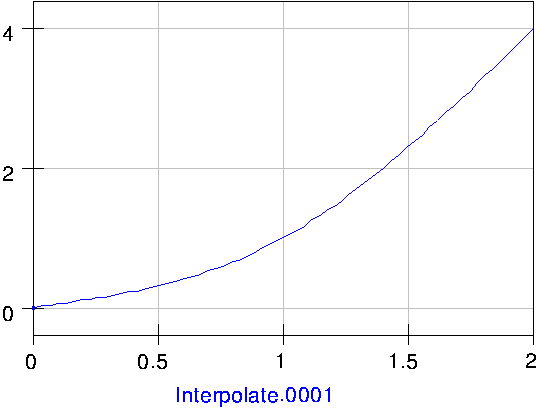
\includegraphics[%
  width=.5\linewidth]{interpolate_example}\end{center}


\caption{Interpolated curve}
\end{figure}


Use the Cartesian diagram to display it.

\begin{description}
\item [See~also]~
\end{description}
\textcolor{blue}{\hyperlink{sum}{sum()}}\textcolor{black}{,} \textcolor{blue}{\hyperlink{prod}{prod()}}


\newpage
\subsubsection*{\hypertarget{prod}{}{\Large prod\index{prod}()}}


\paragraph{\label{par:Prod}Product of vector elements.}

\begin{description}
\item [Syntax]~
\end{description}
y=prod(x)

\begin{description}
\item [Arguments]~
\end{description}
\begin{tabular}{|c|c|c|c|}
\hline 
Name&
Type&
Def. Range&
Required\tabularnewline
\hline
\hline 
x&
$\mathbb{R}$, $\mathbb{C}$, $\mathbb{R}^{n}$, $\mathbb{C}^{n}$&
$\left]-\infty,+\infty\right[$&
$\surd$\tabularnewline
\hline
\end{tabular}

\begin{description}
\item [Description]~
\end{description}
This function returns the product of the elements of a real or complex
vector.

\medskip{}
For $x\in$$\mathbb{C}^{n}$: $y=$$\prod\limits _{i=1}^{n}x_{i}$
\medskip{}

For \textit{x} being a real or complex number, \textit{x} itself is
returned.

\begin{description}
\item [Example]~
\end{description}
\begin{lyxlist}{00.00.0000}
\item [\texttt{y=prod(linspace(1,3,10))}]returns 583.
\end{lyxlist}
\begin{description}
\item [See~also]~
\end{description}
\textcolor{blue}{\hyperlink{sum}{sum()}}\textcolor{black}{,} \textcolor{blue}{\hyperlink{avg}{avg()}}\textcolor{black}{,}
\textcolor{blue}{\hyperlink{max}{max()}}\textcolor{black}{,} \textcolor{blue}{\hyperlink{min}{min()}}


\newpage
\subsubsection*{\hypertarget{sum}{}{\Large sum\index{sum}()}}


\paragraph{\label{par:Sum}Sum of vector elements.}

\begin{description}
\item [Syntax]~
\end{description}
y=sum(x)

\begin{description}
\item [Arguments]~
\end{description}
\begin{tabular}{|c|c|c|c|}
\hline 
Name&
Type&
Def. Range&
Required\tabularnewline
\hline
\hline 
x&
$\mathbb{R}$, $\mathbb{C}$, $\mathbb{R}^{n}$, $\mathbb{C}^{n}$&
$\left]-\infty,+\infty\right[$&
$\surd$\tabularnewline
\hline
\end{tabular}

\begin{description}
\item [Description]~
\end{description}
This function returns the sum of the elements of a real or complex
vector.

\medskip{}
For $x\in$$\mathbb{C}^{n}$: $y=$$\sum\limits _{i=1}^{n}x_{i}$
\medskip{}

For \textit{x} being a real or complex number, \textit{x} itself is
returned.

\begin{description}
\item [Example]~
\end{description}
\begin{lyxlist}{00.00.0000}
\item [\texttt{y=sum(linspace(1,3,10))}]returns 20.
\end{lyxlist}
\begin{description}
\item [See~also]~
\end{description}
\textcolor{blue}{\hyperlink{prod}{prod()}}\textcolor{black}{,} \textcolor{blue}{\hyperlink{avg}{avg()}}\textcolor{black}{,}
\textcolor{blue}{\hyperlink{max}{max()}}\textcolor{black}{,} \textcolor{blue}{\hyperlink{min}{min()}}


\newpage
\subsubsection*{\hypertarget{xvalue}{}{\Large xvalue\index{xvalue}()}}


\paragraph{\label{par:xvalue}Returns x-value which is associated with the y-value
nearest to a specified y-value in a given vector.}

\begin{description}
\item [Syntax]~
\end{description}
x=xvalue(f,yval)

\begin{description}
\item [Arguments]~
\end{description}
\begin{tabular}{|c|c|c|c|}
\hline 
Name&
Type&
Def. Range&
Required\tabularnewline
\hline
\hline 
f&
$\mathbb{R}^{n}$, $\mathbb{C}^{n}$&
$\left]-\infty,+\infty\right[$&
$\surd$\tabularnewline
\hline
yval&
$\mathbb{R}$, $\mathbb{C}$&
$\left]-\infty,+\infty\right[$&
$\surd$\tabularnewline
\hline
\end{tabular}

\begin{description}
\item [Description]~
\end{description}
This function returns the \textit{x}-value which is associated with
the \textit{y}-value nearest to \textit{yval} in the given vector
\textit{f}; therefore the vector \textit{f} must have a single data
dependency.

\begin{description}
\item [Example]~
\end{description}
\begin{lyxlist}{00.00.0000}
\item [\texttt{x=xvalue(f,1)}.]~
\end{lyxlist}
\begin{description}
\item [See~also]~
\end{description}
\textcolor{blue}{\hyperlink{yvalue}{yvalue()}}\textcolor{black}{,}
\textcolor{blue}{\hyperlink{interpolate}{interpolate()}}


\newpage
\subsubsection*{\hypertarget{yvalue}{}{\Large yvalue\index{yvalue}()}}


\paragraph{\label{par:yvalue}Returns y-value of a given vector which is located
nearest to the specified x-value.}

\begin{description}
\item [Syntax]~
\end{description}
y=yvalue(f,xval)

\begin{description}
\item [Arguments]~
\end{description}
\begin{tabular}{|c|c|c|c|}
\hline 
Name&
Type&
Def. Range&
Required\tabularnewline
\hline
\hline 
f&
$\mathbb{R}^{n}$, $\mathbb{C}^{n}$&
$\left]-\infty,+\infty\right[$&
$\surd$\tabularnewline
\hline
xval&
$\mathbb{R}$, $\mathbb{C}$&
$\left]-\infty,+\infty\right[$&
$\surd$\tabularnewline
\hline
\end{tabular}

\begin{description}
\item [Description]~
\end{description}
This function returns the y-value of the given vector \textit{f} which
is located nearest to the x-value \textit{xval}; therefore the vector
\textit{f} must have a single data dependency.

\begin{description}
\item [Example]~
\end{description}
\begin{lyxlist}{00.00.0000}
\item [\texttt{y=yvalue(f,1)}.]~
\end{lyxlist}
\begin{description}
\item [See~also]~
\end{description}
\textcolor{blue}{\hyperlink{xvalue}{xvalue()}}\textcolor{black}{,}
\textcolor{blue}{\hyperlink{interpolate}{interpolate()}}


\newpage
\tutsubsubsection{\label{sub:Differentiation-and-Integration}Differentiation and Integration}

\subsubsection*{\hypertarget{ddx}{}{\Large ddx\index{ddx}()}}


\paragraph{\label{par:Differentiate-Symbolicly}Differentiate mathematical expression with respect to a given variable.}

\begin{description}
\item [Syntax]~
\end{description}
y=ddx(f(x),x)

\begin{description}
\item [Arguments]~
\end{description}
\begin{tabular}{|c|c|c|c|c|}
\hline 
Name&
Type&
Def. Range&
Required&
Default\tabularnewline
\hline
\hline 
f(x)&
&
&
$\surd$&
\tabularnewline
\hline 
x&
$\mathbb{R}$, $\mathbb{C}$, $\mathbb{R}^{m}$, $\mathbb{C}^{m}$&
$\left]-\infty,+\infty\right[$&
$\surd$&
\tabularnewline
\hline 
\end{tabular}

\begin{description}
\item [Description]~
\end{description}
This function executes a symbolic differentiation on a function \textit{f(x)} with respect to a variable \textit{x}.
The result is evaluated at the contents $x_0$ of \textit{x}.

\medskip{}
${\displaystyle y=\frac{df}{dx} \Bigg|_{x_0}}$
\medskip{}

If \textit{x} is a vector, the differential quotient is evaluated for all components of \textit{x}, giving a result vector \textit{y}.

\begin{description}
\item [Example]~
\end{description}
Create a vector \textit{x} by setting \texttt{x=linspace(0,2,3)}, thus $x=\left[0,1,2\right]^T$. Entering
\begin{lyxlist}{00.00.0000}
\item [\texttt{y=ddx(sin(x),x}]returns 1, 0.54, -0.416.
\end{lyxlist}
Why? ${\displaystyle \frac{df}{dx}=\frac{d \sin(x)}{dx}=\cos(x)}$, and $\cos(x)$ evaluated at $x=\left[0,1,2\right]^T$
gives the result above.
\begin{description}
\item [See~also]~
\end{description}
\textcolor{blue}{\hyperlink{diff}{diff()}}

\newpage
\subsubsection*{\hypertarget{diff}{}{\Large diff\index{diff}()}}


\paragraph{\label{par:Differentiate}Differentiate vector with respect to another
vector.}

\begin{description}
\item [Syntax]~
\end{description}
z=diff(y,x,n)

\begin{description}
\item [Arguments]~
\end{description}
\begin{tabular}{|c|c|c|c|c|}
\hline 
Name&
Type&
Def. Range&
Required&
Default\tabularnewline
\hline
\hline 
y&
$\mathbb{R}^{k}$, $\mathbb{C}^{k}$&
$\left]-\infty,+\infty\right[$&
$\surd$&
\tabularnewline
\hline 
x&
$\mathbb{R}^{m}$, $\mathbb{C}^{m}$&
$\left]-\infty,+\infty\right[$&
$\surd$&
\tabularnewline
\hline 
n&
$\mathbb{N}$&
&
&
1\tabularnewline
\hline
\end{tabular}

\begin{description}
\item [Description]~
\end{description}
This function numerically differentiates a vector \textit{y} with
respect to a vector \textit{x}. If the optional integer parameter
\textit{n} is given, the n-th derivative is calculated. Differentiation
is executed for \textit{N=}min\textit{(k,m)} elements. For n=1,

\medskip{}
${\displaystyle \frac{\Delta y_{i}}{\Delta x_{i}}}=$$\left\{ \begin{array}{cc}
{\displaystyle \frac{1}{2}\left(\frac{y_{i}-y_{i-1}}{x_{i}-x_{i-1}}+\frac{y_{i+1}-y_{i}}{x_{i+1}-x_{i}}\right)} & \textrm{for}\: N-1>i>0\\
{\displaystyle \frac{y_{i+1}-y_{i}}{x_{i+1}-x_{i}}} & \textrm{for}\: i=0\\
{\displaystyle \frac{y_{i}-y_{i-1}}{x_{i}-x_{i-1}}} & \textrm{for}\: i=N-1\end{array}\right.$
\medskip{}

If \textit{n>1}, the result of the differentiation above
is assigned to \textit{y} and the aforementioned differentiation step
is repeated until the number of those steps is equal to \textit{n}.

\begin{description}
\item [Example]~
\end{description}
\begin{lyxlist}{00.00.0000}
\item [\texttt{z=diff(linspace(1,3,3),linspace(2,3,3))}]returns 2, 2, 2.
\end{lyxlist}
\begin{description}
\item [See~also]~
\end{description}
\textcolor{blue}{\hyperlink{integrate}{integrate()}}\textcolor{black}{,}
\textcolor{blue}{\hyperlink{sum}{sum()}}\textcolor{black}{,} \textcolor{blue}{\hyperlink{max}{max()}}\textcolor{black}{,}
\textcolor{blue}{\hyperlink{min}{min()}}


\newpage
\subsubsection*{\hypertarget{integrate}{}{\Large integrate\index{integrate}()}}


\paragraph{\label{par:Integrate}Integrate vector.}

\begin{description}
\item [Syntax]~
\end{description}
z=integrate(y,h)

\begin{description}
\item [Arguments]~
\end{description}
\begin{tabular}{|c|c|c|c|}
\hline 
Name&
Type&
Def. Range&
Required\tabularnewline
\hline
\hline 
y&
$\mathbb{R}$, $\mathbb{C}$, $\mathbb{R}^{n}$, $\mathbb{C}^{n}$&
$\left]-\infty,+\infty\right[$&
$\surd$\tabularnewline
\hline 
h&
$\mathbb{R}$, $\mathbb{C}$&
$\left]-\infty,+\infty\right[$&
$\surd$\tabularnewline
\hline
\end{tabular}

\begin{description}
\item [Description]~
\end{description}
This function numerically integrates a vector \textit{x} with respect
to a differential \textit{h}. The integration method is according
to the trapezoidal rule:

\medskip{}
$\int f\left(t\right)dt\approx h\,\left({\displaystyle \frac{y_{0}}{2}}+y_{1}+y_{2}+\ldots+y_{n-1}+{\displaystyle \frac{y_{n}}{2}}\right)$
\medskip{}

\begin{description}
\item [Example]~
\end{description}
Calculate an approximation of the integral $\int\limits _{1}^{3}t\, dt$
using 101 points:

\begin{lyxlist}{00.00.0000}
\item [\texttt{z=integrate(linspace(1,3,101))}]returns
4.
\end{lyxlist}
\begin{description}
\item [See~also]~
\end{description}
\textcolor{blue}{\hyperlink{diff}{diff()}}\textcolor{black}{,} \textcolor{blue}{\hyperlink{sum}{sum()}}\textcolor{black}{,}
\textcolor{blue}{\hyperlink{max}{max()}}\textcolor{black}{,} \textcolor{blue}{\hyperlink{min}{min()}}


\newpage
\tutsubsubsection{\label{sub:Signal-Processing}Signal Processing}


\subsubsection*{\hypertarget{dft}{}{\Large dft\index{dft}()}}


\paragraph{\label{par:Discrete-Fourier-Transform}Discrete Fourier Transform.}

\begin{description}
\item [Syntax]~
\end{description}
y=dft(v)

\begin{description}
\item [Arguments]~
\end{description}
\begin{tabular}{|c|c|c|c|}
\hline 
Name&
Type&
Def. Range&
Required\tabularnewline
\hline
\hline 
v&
$\mathbb{R}^{n}$, $\mathbb{C}^{n}$&
$\left]-\infty,+\infty\right[$&
$\surd$\tabularnewline
\hline 
\end{tabular}

\begin{description}
\item [Description]~
\end{description}

This function computes the Discrete Fourier Transform (DFT) of a
vector \textit{v}. The advantage of this function compared to
\textcolor{blue}{\hyperlink{fft}{fft()}} \textcolor{black}{is that}
the number \textit{n} of components of
\textit{v} is arbitrary, while for the latter \textit{n} must be a
power of 2. The drawbacks are that dft() is slower and less accurate
than \textcolor{blue}{\hyperlink{fft}{fft()}}.

\begin{description}
\item [Example]~
\end{description}
This calculates the spectrum $y$ of a DC signal:

\begin{lyxlist}{00.00.0000}
\item [\texttt{y=dft(linspace(1,1,7))}]returns \begin{tabular}{|c|}
\hline 
y\tabularnewline
\hline
\hline 
1\tabularnewline
\hline 
-1.59e-17+j1.59e-17\tabularnewline
\hline 
$\vdots$\tabularnewline
\hline 
2.22e-16-j1.11e-16\tabularnewline
\hline
\end{tabular}
\end{lyxlist}
Please note that in this example 7 points are used for the time vector
v. Since 7 is not a power of 2, the same expression used together with
the fft() function would lead to wrong results. Note also the rounding
errors where {}``0'' would be the correct value.

\begin{description}
\item [See~also]~
\end{description}
\textcolor{blue}{\hyperlink{idft}{idft()}}\textcolor{black}{,} \textcolor{blue}{\hyperlink{fft}{fft()}}\textcolor{black}{,}
\textcolor{blue}{\hyperlink{ifft}{ifft()}}\textcolor{black}{,}
\textcolor{blue}{\hyperlink{Freq2Time}{Freq2Time()}}\textcolor{black}{,}
\textcolor{blue}{\hyperlink{Time2Freq}{Time2Freq()}}


\newpage
\subsubsection*{\hypertarget{fft}{}{\Large fft\index{fft}()}}


\paragraph{\label{par:Fast-Fourier-Transform}Fast Fourier Transform.}

\begin{description}
\item [Syntax]~
\end{description}
y=fft(v)

\begin{description}
\item [Arguments]~
\end{description}
\begin{tabular}{|c|c|c|c|}
\hline 
Name&
Type&
Def. Range&
Required\tabularnewline
\hline
\hline 
v&
$\mathbb{R}^{n}$, $\mathbb{C}^{n}$&
$\left]-\infty,+\infty\right[$&
$\surd$\tabularnewline
\hline 
\end{tabular}

\begin{description}
\item [Description]~
\end{description}
This function computes the Fast Fourier Transform (FFT) of a vector
\textit{v}. The number \textit{n} of components of \textit{v} must be
a power of 2.

\begin{description}
\item [Example]~
\end{description}
This calculates the spectrum $y$ of a DC signal:

\begin{lyxlist}{00.00.0000}
\item [\texttt{y=fft(linspace(1,1,8))}]returns \begin{tabular}{|c|}
\hline 
y\tabularnewline
\hline
\hline 
1\tabularnewline
\hline 
0\tabularnewline
\hline 
$\vdots$\tabularnewline
\hline 
0\tabularnewline
\hline
\end{tabular}
\end{lyxlist}
\begin{description}
\item [See~also]~
\end{description}
\textcolor{blue}{\hyperlink{ifft}{ifft()}}\textcolor{black}{,} \textcolor{blue}{\hyperlink{dft}{dft()}}\textcolor{black}{,}
\textcolor{blue}{\hyperlink{idft}{idft()}}\textcolor{black}{,}
\textcolor{blue}{\hyperlink{Freq2Time}{Freq2Time()}}\textcolor{black}{,}
\textcolor{blue}{\hyperlink{Time2Freq}{Time2Freq()}}\textcolor{black}{,}
\textcolor{blue}{\hyperlink{fftshift}{fftshift()}}


\newpage
\subsubsection*{\hypertarget{idft}{}{\Large idft\index{idft}()}}


\paragraph{\label{par:Inverse-Discrete-Fourier}Inverse Discrete Fourier Transform.}

\begin{description}
\item [Syntax]~
\end{description}
y=idft(v)

\begin{description}
\item [Arguments]~
\end{description}
\begin{tabular}{|c|c|c|c|}
\hline 
Name&
Type&
Def. Range&
Required\tabularnewline
\hline
\hline 
v&
$\mathbb{R}^{n}$, $\mathbb{C}^{n}$&
$\left]-\infty,+\infty\right[$&
$\surd$\tabularnewline
\hline 
\end{tabular}

\begin{description}
\item [Description]~
\end{description}
This function computes the Inverse Discrete Fourier Transform (IDFT)
of a vector \textit{v}.  The advantage of this function compared to
\textcolor{blue}{\hyperlink{ifft}{ifft()}}
\textcolor{black}{is that} the number \textit{n} of components of
\textit{v} is arbitrary, while for the latter \textit{n} must be a
power of 2. The drawbacks are that idft() is slower and less accurate
than \textcolor{blue}{\hyperlink{ifft}{ifft()}}.

\begin{description}
\item [Example]~
\end{description}
This calculates the time function $y$ belonging to a white spectrum:

\begin{lyxlist}{00.00.0000}
\item [\texttt{y=idft(linspace(1,1,7))}]returns \begin{tabular}{|c|}
\hline 
y\tabularnewline
\hline
\hline 
7\tabularnewline
\hline 
-1.11e-16-j1.11e-16\tabularnewline
\hline 
$\vdots$\tabularnewline
\hline 
1.55e-15+j7.77e-16\tabularnewline
\hline
\end{tabular}
\end{lyxlist}
Please note that in this example 7 points are used for the spectrum
vector v. Since 7 is not a power of 2, the same expression used
together with the ifft() function would lead to wrong results. Note
also the rounding errors where {}``0'' would be the correct value.

\begin{description}
\item [See~also]~
\end{description}
\textcolor{blue}{\hyperlink{dft}{dft()}}\textcolor{black}{,} \textcolor{blue}{\hyperlink{ifft}{ifft()}}\textcolor{black}{,}
\textcolor{blue}{\hyperlink{fft}{fft()}}\textcolor{black}{,}
\textcolor{blue}{\hyperlink{Freq2Time}{Freq2Time()}}\textcolor{black}{,}
\textcolor{blue}{\hyperlink{Time2Freq}{Time2Freq()}}\textcolor{black}{,}
\textcolor{blue}{\hyperlink{fftshift}{fftshift()}}


\newpage
\subsubsection*{\hypertarget{ifft}{}{\Large ifft\index{ifft}()}}


\paragraph{\label{par:Inverse-Fast-Fourier}Inverse Fast Fourier Transform.}

\begin{description}
\item [Syntax]~
\end{description}
y=ifft(v)

\begin{description}
\item [Arguments]~
\end{description}
\begin{tabular}{|c|c|c|c|}
\hline 
Name&
Type&
Def. Range&
Required\tabularnewline
\hline
\hline 
v&
$\mathbb{R}^{n}$, $\mathbb{C}^{n}$&
$\left]-\infty,+\infty\right[$&
$\surd$\tabularnewline
\hline 
\end{tabular}

\begin{description}
\item [Description]~
\end{description}
This function computes the Inverse Fast Fourier Transform (IFFT) of a
vector \textit{v}.  The number \textit{n} of components of \textit{v}
must be a power of 2.

\begin{description}
\item [Example]~
\end{description}
This calculates the time function $y$ belonging to a white spectrum:

\begin{lyxlist}{00.00.0000}
\item [\texttt{y=ifft(linspace(1,1,8))}]returns \begin{tabular}{|c|}
\hline 
y\tabularnewline
\hline
\hline 
8\tabularnewline
\hline 
0\tabularnewline
\hline 
$\vdots$\tabularnewline
\hline 
0\tabularnewline
\hline
\end{tabular}
\end{lyxlist}
\begin{description}
\item [See~also]~
\end{description}
\textcolor{blue}{\hyperlink{fft}{fft()}}\textcolor{black}{,} \textcolor{blue}{\hyperlink{dft}{dft()}}\textcolor{black}{,}
\textcolor{blue}{\hyperlink{idft}{idft()}}\textcolor{black}{,}
\textcolor{blue}{\hyperlink{Freq2Time}{Freq2Time()}}\textcolor{black}{,}
\textcolor{blue}{\hyperlink{Time2Freq}{Time2Freq()}}\textcolor{black}{,}
\textcolor{blue}{\hyperlink{fftshift}{fftshift()}}



\newpage
\subsubsection*{\hypertarget{fftshift}{}{\Large fftshift\index{fftshift}()}}


\paragraph{\label{par:fftshift}Move the frequency 0 to the center of the FFT vector.}

\begin{description}
\item [Syntax]~
\end{description}
y=fftshift(v)

\begin{description}
\item [Arguments]~
\end{description}
\begin{tabular}{|c|c|c|c|}
\hline 
Name&
Type&
Def. Range&
Required\tabularnewline
\hline
\hline 
v&
$\mathbb{R}^{n}$, $\mathbb{C}^{n}$&
$\left]-\infty,+\infty\right[$&
$\surd$\tabularnewline
\hline 
\end{tabular}

\begin{description}
\item [Description]~
\end{description}
This function shuffles the FFT values of vector \textit{v} in order to move the frequency 0 to the center of the vector.
Below of it the components with negative frequencies are located, above those with positive frequencies.
Herewith the "classical" look of a spectrum as gained by a spectrum analyzer is obtained.

\begin{description}
\item [Example]~
\end{description}
Suppose $x$ to be the result of a FFT of 8 elements, e.g.\begin{tabular}{|c|}
\hline 
x\tabularnewline
\hline
\hline 
1\tabularnewline
\hline 
2\tabularnewline
\hline 
$\vdots$\tabularnewline
\hline 
8\tabularnewline
\hline
\end{tabular}

The result of the FFT is sorted in such a way that the component with frequency zero is the first element (1) of the vector.
The components with positive frequency follow (2,3,4).
After that, the components with negative frequency (5,6,7,8) are arranged, starting from the most negative value.
This pattern can be exemplarily generated in Qucs by writing \texttt{x=linspace(1,8,8)}. Then

\begin{lyxlist}{00.00.0000}
\item [\texttt{y=fftshift(x)}]returns \begin{tabular}{|c|}
\hline 
y\tabularnewline
\hline
\hline 
5\tabularnewline
\hline 
6\tabularnewline
\hline 
7\tabularnewline
\hline
8\tabularnewline
\hline
1\tabularnewline
\hline
2\tabularnewline
\hline
3\tabularnewline
\hline
4\tabularnewline
\hline
\end{tabular}
\end{lyxlist}
As you can see, the component with frequency 0 (element 1) is moved to the middle of the spectrum vector.
Beneath of it the components with negative frequencies appear (5,6,7,8), above those with positive frequencies (2,3,4).

\begin{description}
\item [See~also]~
\end{description}
\textcolor{blue}{\hyperlink{fft}{fft()}}\textcolor{black}{,}
\textcolor{blue}{\hyperlink{ifft}{ifft()}}\textcolor{black}{,} \textcolor{blue}{\hyperlink{dft}{dft()}}\textcolor{black}{,}
\textcolor{blue}{\hyperlink{idft}{idft()}}


\newpage
\subsubsection*{\hypertarget{Time2Freq}{}{\Large Time2Freq\index{Time2Freq}()}}


\paragraph{\label{par:Interpreted-Discrete-Fourier-Transform}Interpreted Discrete Fourier Transform.}

\begin{description}
\item [Syntax]~
\end{description}
y=Time2Freq(v,t)

\begin{description}
\item [Arguments]~
\end{description}
\begin{tabular}{|c|c|c|c|}
\hline 
Name&
Type&
Def. Range&
Required\tabularnewline
\hline
\hline 
v&
$\mathbb{R}^{n}$, $\mathbb{C}^{n}$&
$\left]-\infty,+\infty\right[$&
$\surd$\tabularnewline
\hline 
t&
$\mathbb{R}^{k}$, $\mathbb{C}^{k}$&
$\left]-\infty,+\infty\right[$&
$\surd$\tabularnewline
\hline
\end{tabular}

\begin{description}
\item [Description]~
\end{description}
This function computes the Discrete Fourier Transform (DFT) of a vector
\textit{v} with respect to a time vector \textit{t}.

\begin{description}
\item [Example]~
\end{description}
This calculates the spectrum y(f) of a DC signal:

\begin{lyxlist}{00.00.0000}
\item [\texttt{y=Time2Freq(linspace(1,1,7),linspace(0,1,2))}]returns\\

\begin{tabular}{|c|c|}
\hline 
Frequency&
y\tabularnewline
\hline
\hline 
0&
1\tabularnewline
\hline 
0.167&
-1.59e-17+j1.59e-17\tabularnewline
\hline 
$\vdots$&
$\vdots$\tabularnewline
\hline 
1&
2.22e-16-j1.11e-16\tabularnewline
\hline
\end{tabular}
\end{lyxlist}
Please note that in this example 7 points are used for the time vector
$v$.  Note also the rounding errors at t>0, where {}``0'' would be the
correct value.

\begin{description}
\item [See~also]~
\end{description}
\textcolor{blue}{\hyperlink{idft}{idft()}}\textcolor{black}{,} \textcolor{blue}{\hyperlink{fft}{fft()}}\textcolor{black}{,}
\textcolor{blue}{\hyperlink{ifft}{ifft()}}\textcolor{black}{,}
\textcolor{blue}{\hyperlink{Freq2Time}{Freq2Time()}}

\newpage
\subsubsection*{\hypertarget{Freq2Time}{}{\Large Freq2Time\index{Freq2Time}()}}


\paragraph{\label{par:Interpreted-Inverse-Discrete-Fourier}Interpreted Inverse Discrete Fourier Transform.}

\begin{description}
\item [Syntax]~
\end{description}
y=Freq2Time(v,f)

\begin{description}
\item [Arguments]~
\end{description}
\begin{tabular}{|c|c|c|c|}
\hline 
Name&
Type&
Def. Range&
Required\tabularnewline
\hline
\hline 
v&
$\mathbb{R}^{n}$, $\mathbb{C}^{n}$&
$\left]-\infty,+\infty\right[$&
$\surd$\tabularnewline
\hline 
f&
$\mathbb{R}^{k}$, $\mathbb{C}^{k}$&
$\left]-\infty,+\infty\right[$&
$\surd$\tabularnewline
\hline
\end{tabular}

\begin{description}
\item [Description]~
\end{description}
This function computes the Inverse Discrete Fourier Transform (IDFT)
of a vector \textit{v} with respect to a frequency vector \textit{f}.

\begin{description}
\item [Example]~
\end{description}
This calculates the time function y(t) belonging to a white spectrum:

\begin{lyxlist}{00.00.0000}
\item [\texttt{y=Freq2Time(linspace(1,1,7),linspace(0,1,2))}]returns\\

\begin{tabular}{|c|c|}
\hline 
Frequency&
y\tabularnewline
\hline
\hline 
0&
7\tabularnewline
\hline 
0.167&
-1.11e-16-j1.11e-16\tabularnewline
\hline 
$\vdots$&
$\vdots$\tabularnewline
\hline 
1&
1.55e-15+j7.77e-16\tabularnewline
\hline
\end{tabular}
\end{lyxlist}
Please note that in this example 7 points are used for the spectrum
vector $v$.  Note also the rounding errors at t>0, where {}``0'' would
be the correct value.

\begin{description}
\item [See~also]~
\end{description}
\textcolor{blue}{\hyperlink{dft}{dft()}}\textcolor{black}{,} \textcolor{blue}{\hyperlink{ifft}{ifft()}}\textcolor{black}{,}
\textcolor{blue}{\hyperlink{fft}{fft()}}\textcolor{black}{,}
\textcolor{blue}{\hyperlink{Time2Freq}{Time2Freq()}}

\newpage
\subsubsection*{\hypertarget{kbd}{}{\Large kbd\index{kbd}()}}


\paragraph{\label{par:Kaiser-Bessel-window}Kaiser-Bessel derived window.}

\begin{description}
\item [Syntax]~
\end{description}
y=kbd(a,n)

y=kbd(a)

\begin{description}
\item [Arguments]~
\end{description}
\begin{tabular}{|c|c|c|c|c|}
\hline 
Name&
Type&
Def. Range&
Required&
Default\tabularnewline
\hline
\hline 
a&
$\mathbb{R}$&
$\left]-\infty,+\infty\right[$&
$\surd$&
\tabularnewline
\hline 
n&
$\mathbb{N}$&
$\left[1,+\infty\right[$&
&
64\tabularnewline
\hline
\end{tabular}

\begin{description}
\item [Description]~
\end{description}
This function generates a Kaiser-Bessel window according to

\medskip{}
$y_{k}\quad\,=\:{\displaystyle \sqrt{\frac{\sum\limits _{i=0}^{k}I_{0}\left(\pi\, a\,\sqrt{1-\left(\frac{4\, i}{n}-1\right)}\right)}{\sum\limits _{i=0}^{\frac{n}{2}}I_{0}\left(\pi\, a\,\sqrt{1-\left(\frac{4\, i}{n}-1\right)}\right)}}}$,
\medskip{}

$y_{n-k-1}=\: y_{k}$
\medskip{}

for $0\leq k<\frac{n}{2}$
\medskip{}

If the parameter \textit{n} is not specified, \textit{n}=64
is assumed.

\begin{description}
\item [Example]~
\end{description}
\begin{lyxlist}{00.00.0000}
\item [\texttt{y=kbd(0.1,4)}]returns .
\end{lyxlist}
\begin{description}
\item [See~also]~
\end{description}
\textcolor{blue}{\hyperlink{dft}{dft()}}\textcolor{black}{,} \textcolor{blue}{\hyperlink{ifft}{ifft()}}\textcolor{black}{,}
\textcolor{blue}{\hyperlink{fft}{fft()}}
